
\documentclass[twoside,12pt,a4paper]{report}

% Math
\usepackage{amsfonts}
\usepackage{amsmath}

% Margins
\usepackage[top=2.4cm,bottom=2.4cm,outer=2.4cm,inner=4.2cm]{geometry}

% Standalone
\usepackage{standalone}

%TiKz
\usepackage{tikz}
\usetikzlibrary{positioning}
\usetikzlibrary{arrows}
\usetikzlibrary{shapes}
\usetikzlibrary{calc}

% Appendices
\usepackage[toc,page]{appendix}

% SidewaysFigure
\usepackage{rotating}

% Multi-page Tables
\usepackage{longtable}

% CMU sans serif font.
\usepackage[T1]{fontenc}
\renewcommand*\familydefault{\sfdefault}

% Hyperlinks
\usepackage{hyperref}
\hypersetup{
    colorlinks=true,       	% false: boxed links; true: colored links
    linkcolor=black,          	% color of internal links (change box color with linkbordercolor)
    citecolor=black,        	% color of links to bibliography
    filecolor=blue,      		% color of file links
    urlcolor=blue           	% color of external links
}

% APA 6 citation and bibliography style % Note: Must be loaded after hyperref
\usepackage{apacite} 

% Abbreviations
\usepackage[acronym]{glossaries}
\makeglossaries
\newacronym{pisa}{PISA}{Programme for International Student Assessment}
\newacronym{oecd}{OECD}{Organisation for Economic Co-operation and Development}
\newacronym{stem}{STEM}{Science, Technology, Engineering and Mathematics}
\newacronym{fmri}{fMRI}{functional magnetic resonance imaging}
\newacronym{naplan}{NAPLAN}{National Assessment Program --- Literacy and Numeracy}
\newacronym{mars}{MARS}{Maths Anxiety Rating Scale}
\newacronym{mas-r}{MAS-R}{Maths Anxiety Scale --- Revised}
\newacronym{ptsd}{PTSD}{Post-Traumatic Stress Disorder}

\newacronym{ac}{AC}{Australian Curriculum}
\newacronym{sace}{SACE}{South Australian Certificate of Education}
\newacronym{amsi}{AMSI}{Australian Mathematical Sciences Institute}

\newacronym{uofa}{UofA}{University of Adelaide}
\newacronym{ecms}{ECMS}{Faculty of Engineering, Computer and Mathematical Sciences}
\newacronym{mlc}{MLC}{Maths Learning Centre}


% Date by Month for Title Page
\usepackage{datetime}
\newdateformat{monthyeardate}{%
  \monthname[\THEMONTH], \THEYEAR}

% Intentionally Blank Page
\newcommand*{\intentionallyblankpage}{
  \vspace*{\fill}
  {\centering \textit{This page intentionally left blank.} \par}
  \vspace{\fill}}
\makeatletter
\renewcommand*{\cleardoublepage}{\clearpage\if@twoside \ifodd\c@page\else
  \intentionallyblankpage
  % \thispagestyle{empty}
  \newpage
  \if@twocolumn\hbox{}\newpage\fi\fi\fi}
\makeatother

% Table of Contents
%\usepackage[nottoc]{tocbibind}
\setcounter{tocdepth}{1}

% Section and Figure Numbering
%\renewcommand\thesection{\arabic{section}}
%\usepackage{chngcntr}
%\counterwithout{figure}{chapter}
%\counterwithout{table}{chapter}

% Referencing Commands
\newcommand{\refchap}[1]{\hyperref[chap:#1]{Chapter~\ref{chap:#1}}}
\newcommand{\refsec}[1]{\hyperref[sec:#1]{Section~\ref{sec:#1}}}
\newcommand{\reffig}[1]{\hyperref[fig:#1]{Figure~\ref{fig:#1}}}
\newcommand{\reftab}[1]{\hyperref[tab:#1]{Table~\ref{tab:#1}}}
\newcommand{\refapp}[1]{\hyperref[app:#1]{Appendix~\ref{app:#1}}}




\begin{document}



%-----beginning of title page -----------------------------
\begin{titlepage}

\begin{flushleft}
\null
\vspace{2 cm}
\hrule
\vspace{1 cm}
{\huge{\bf MathsStart and MathsTrack: \\[2pt] Mathematics Bridging at \\[6pt] the University of Adelaide.}}
\vspace*{2cm}

\vspace{5.5 cm}
{\large by Dr. Lyron Juan Winderbaum}\\
\vspace{1 cm}
{\large Primary Supervisor: Dr. Igusti Darmawan}\\
\vspace{0.5 cm}
{\large Co - Supervisors: Dr. David Butler and Nicholas Crouch}\\
\vspace{2 cm}
{ Thesis submitted in partial fulfilment of the requirements for the degree of Master of Teaching (EDUC 7557)}\\
\vspace{0.5 cm}
\end{flushleft}

\begin{flushright}
{\monthyeardate\today }
\end{flushright}

\vspace{0.5 cm}
\hrule
\vspace{0.65cm}

\begin{flushleft}
\textbf{SCHOOL OF EDUCATION}
\end{flushleft}
\vspace{-1.5cm}
% University of Adelaide Crest
\begin{flushright}
\includegraphics[scale=0.75]{./files/UoA_logo_col_vert.png}
\end{flushright}
\vspace{-2 cm}

\end{titlepage}
%---------- end of title page -------------------------------



\pagenumbering{roman}



%---------------- table of contents -------------------------
\setcounter{page}{2}
\intentionallyblankpage
\newpage
\intentionallyblankpage
\tableofcontents
\addcontentsline{toc}{chapter}{Contents}
%---------------- end of TOC -------------------------



%%---------------- Glossary ----------------------------------
%% \setglossarystyle{mcolindex}
\glsaddall
%\newpage
%\cleardoublepage
%\intentionallyblankpage
\printglossaries
\addcontentsline{toc}{chapter}{Acronyms}
%%---------------- end of Glossary ---------------------------



% --------------- Abstract ----------------------------------
\glsresetall
\cleardoublepage
\chapter*{Abstract}
\addcontentsline{toc}{chapter}{Abstract}

In this thesis the University of Adelaide's mathematics bridging courses: MathsStart and MathsTrack are discussed in detail. Their context and purpose is reviewed, their content is aligned to national and state highschool curriculums, as well as appropriate entry-level university courses. The pedagogy and excellence in educational practice demonstrated through the University of Adelaide's maths learning center, which offers these bridging courses, is examined with an eye to learning from their exemplary approach to supporting what can be one of the most vunerable cohorts of students attempting to enter into tertiary education. Ultimately, reccomendations are made both in terms of exemplary practice that can be generalised to other such courses accross Australia, and also in terms of restructuring of the courses to better align them with national and state curriculums, while also tailoring their content to better suit the cohort of students enrolling in these courses.

% --------------- end of abstract ---------------------------



%---------- publications page -------------------------------
% \cleardoublepage
% \chapter*{Publications and Presentations}
% \addcontentsline{toc}{chapter}{Publications and Presentations}
% 
% \lipsum[1-3]
%---------- end of publications -----------------------------



%---------- declaration page --------------------------------
\cleardoublepage
\chapter*{Declaration}
\addcontentsline{toc}{chapter}{Declaration}

I certify that this work contains no material which has been accepted 
for the award of any other degree or diploma in my name, in any
university or other tertiary institution and, to the best of my knowledge 
and belief, contains no material previously published or written
by another person, except where due reference has been made in the 
text. In addition, I certify that no part of this work will, in the
future, be used in a submission in my name, for any other degree or 
diploma in any university or other tertiary institution without the
prior approval of the University of Adelaide and where applicable, any 
partner institution responsible for the joint-award of this degree.

I give permission for the digital version of my thesis to be made 
available on the web, via the University’s digital research repository,
the Library Search and also through web search engines.

\vspace{2cm}

\begin{flushleft}
Signed:  \\[15 pt]
Date:
\end{flushleft}

% \vspace{20 pt}
% \begin{flushleft}
% Signed  by supervisor:\\[15 pt]
% Date:
% \end{flushleft}

%---------- end of declaration page -------------------------



%---------- acknowledgements page ---------------------------
\cleardoublepage
\chapter*{Acknowledgements}
\addcontentsline{toc}{chapter}{Acknowledgements}

First, my thanks go to David Butler and Nicholas Crouch from the maths learning center at the University of Adelaide.
Not only did their exemplary educatational expertise inspire me to try my hand at education in the first place, but they 
continue to inspire me on a daily basis with the way the help and support students. Even while dealing with a university review Nicholas still found time (somehow) to sit with me and discuss improvements that could be made to their bridging courses. 

My thanks also extend to Igusti Darmawan, my supervisor from inside the school of education, for his guidance but mostly support and his willingness to allow me to pursue a somewhat unorthodox project of my own construction, despite it being quite outside of his speciality area of educational research, none-the-less supporting me in my project.

\begin{itemize}
	\item Lynda 
	\item Linda
	\item Brendan, for doing his best,
	\item Ed 
	\item Saman?
	\item Jason?
	\item Amanda?
	\item Trev?
	\item Students?
	\item ...
\end{itemize}

%---------- end of acknowledgments page ---------------------




\cleardoublepage
\chapter{Introduction}
\label{chap:intro}

% Main Body LaTeX settings
\glsresetall
% \setlength{\parindent}{0pt}
% \setlength{\parskip}{2ex plus 0.5ex minus 0.5ex}
\pagenumbering{arabic}

This thesis is concerned with the mathematics bridging courses offered at the \gls{uofa} through the \gls{mlc}: MathsStart and MathsTrack. These courses are intended to take students with very little mathematics background and help them transition into tertiary education (which will generally have some mathematics pre-requisites or assumed knowledge) and be successful. MathsStart and MathsTrack are structured to be student-paced, with no deadlines having been set \textit{apriori}, in a deliberate attempt to both alleiviate test-anxiety, and to aclimitise students to a learning environment in which the primary onus for motivation is on the students. Although the bridging courses are offered through the \gls{mlc} at the \gls{uofa}, the cohort of students come from a very diverse set of backgrounds and have a variety of needs. The majority of students enrolling in these courses are planning to continue into tertiary education at the \gls{uofa}, but many students do not intend to continue into tertiary education at all, and instead enroll in the bridging courses to meet the requisite assumed knowledge for other pathways --- pilot training in the defence forces, for example. 

The continuing decline of interest in mathematics along with the sustained trend of increased demand for mathematically skilled graduates by several major leading industries in Australia and globally (enginneering, science, technology, ...) means that bridging courses playing an increasingly important role in our education system (see \refchap{literature} for a more detailed discussion). Although MathsStart and MathsTrack have been very successful so far, as educators we are continually engaging in reflective practice and looking for ways to improve our teaching practice. It is in this frame of mind, and with the knowledge that comprehensive review of the purpose, structure, and content of MathsStart and MathsTrack has not been done before, the coordinators of the \gls{mlc} directed this work to examine the ``guiding question'':

\begin{quote}
	How can MathsStart and MathsTrack be improved?
\end{quote}

Naturally, this vague statement invites questions such as ``how is improvement measured?'', and ``improvement in what outcome?''. The question is left deliberately vague in this way because part of this work will be dedicated to teasing apart the different possible interpretations, the importance of taking care when interpreting improvement in an educational context, and the consequences of different interpretations. A solution is not proposed, only alternatives and their consequences, with comments on the stakeholders in each case. One important perspective of this question that will be represented heavily in this thesis can be shown by a re-phrasing of the question: 

\begin{quote}
	How can MathsStart and MathsTrack best help the students enrolling in them to be successful going forward?
\end{quote}

Of course this does not neccessarily make the question any less vague --- determining what is in the best interests of our students, is not always clear or straightforward. Nonetheless, this question will be the primary focus of this thesis and despite not being able to give any definitive answers, some suggestions will be made, and at the very least, some context will be given for better understanding the question. Also important to note that although the focus of this work is the courses MathsStart and MathsTrack, much of the contextual background presented herein is relevant to bridging courses accross Australia and internationally. Although it is not the primary goal of this work, giving some broad structure and perhaps a framework for understanding the needs of students going into mathematics bridging programs globally could be thought of as a secondary (perhaps ancillary) objective of this work.

In order to address this guiding question, this thesis will be structured as follows:
\begin{itemize}
	\item The remainder of this introductory chapter (\refchap{intro}) is broken into two sections. First, the purpose, structure, and context of mathematics bridging courses is explored in more detail both in general, and in the specific context of the \gls{uofa} (\refsec{context}). Second, a broad educational framework is introduced in \refsec{framework} which can be used to give large-scale context for the work that will be done in this thesis, motivating the structure of the work and outlining the key areas of importance.
	\item \refchap{methodology} provides a brief description of the methodology employed in the research that will be presented in Chapters~\ref{chap:literature} and \ref{chap:curriculum}.
	\item An indepth discussion of the existing literature is presented in \refchap{literature}: what is known, approaches attempted in the past both in Australia and internationally, frameworks proposed for understanding the secondary-tertiary transition and the maths anxiety-performance link, and some deeper discussion on some of the particularly relevant related concepts.
	\item One of the major contributions of this thesis is the detailed curriculum mapping which is the focus on \refchap{curriculum} in which the top two levels of senior highschool mathematics in the \gls{ac} and \gls{sace} are mapped to each other, and to the content currently in MathsStart and MathsTrack. Detailed discussion of this mapping also includes commentary on how the content relates to typical entry-level university mathematics courses, and other relevant curriculums. 
	\item Finally, in \refchap{recommendations} the conclusions from this work are summarisd, and in particular the interactions between the differnet avenues of research are consolidated. Additional work done outside of this thesis is discussed, and future work is outlined.
\end{itemize}



\section{Context}
\label{sec:context}

\subsection{Bridging Courses in General}

Students will usually enroll in university mathematics bridging courses because they are required to demonstrate a certain level of mathematical knowledge/ competence before commencing study at university, but either do not meet those requirements, or do but feel a lack of confidence in their abilites and feel like they need to refresh/ revise/ learn some mathematics prior to commencing their studies.

Reasons why these students do not either meet the entry requirements, or feel a lack of confidence in their abilities can be quite varied:
\begin{itemize}
	\item A long period of time may have passed since they last studied mathematics (or studied at all). The number and proportion of so-called ``adult learners'' has been steadily increasing for well over three decades now \cite{Johnson2016, Hardin2008,Murtaugh1999}.
	\item They may have performed poorly in mathematics in highschool.
	\item They may have chosen not to study mathematics at a higher level in highschool.
	\item They may suffer from maths anxiety (which would make them likely to fit into the above two categories as well).
\end{itemize}
	
The role of mathematics bridging courses is to take these students, and:
\begin{itemize}
	\item Bridge their content knowledge so they are prepared for entry level university courses, or other tertiary programs required/ assumed knowledge.
	\item Support the growth of their confidence and self-efficacy surrounding mathematics.
	\item Ultimately prepare them to be successful in their continued tertiary study.
\end{itemize}

The question ``what content should be taught in a university bridging course?'' has dramatically different answers depending on the perspective one takes on what the role of such a bridging course is. Even restricting the question to purely knowledge-based content (excluding critical affective aspects such as self-efficacy):
\begin{itemize}
	\item If you take the perspective that the role of such a course is to fill in the gaps in student's knowledge left from an incomplete or maths-light highschool education, then the content that should be taught would include the final year of highschool curriculum. This approach can be particularly appropriate if you do not know the direction of the students, or if they are potentially planning on continuing study at an interstate university, for example.
	\item If you take the perspective that the role of such a course is to prepare students for the further study they plan on engaging in however, this is quite different. The content relevant to any one student will be dramatically differnet depending on their planned direction. The senior highschool mathematics curriculum is quite general and would certainly contain many topics that would be completely irrelevant to any particular student. 
\end{itemize}
In terms of choosing what content to teach in a university bridging course, the above two competing perspectives will often create tension between each other. There are advantages, disadvantages, and important stakeholders of both perspectives and this unfortunately means that this tension cannot be resolved, but rather that must be balanced --- a compromise found.

As though that wasn't difficult enough, the question of ``what content should be taught in a university bridging course?'' is only one part of the issue. As mentioned above, affective aspects such as self-efficacy are crucially important, and it has been shown that, particularly in maths-heavy subject areas such as \gls{stem} diciplines significant numbers of students dropout within the first two years \cite{House2000, Tsui2007}, and that engagement with mathematics support services such as the \gls{mlc} drop-in centre and bridging courses is an approach proven to be effective in addressing this issue \cite{Lee2008}. Consideration of impacts on these affective aspects of perspectives of mathematics is critical for preparing students to be successful. Content cannot be considered in isolation of these factors, and vice versa, they are fundamentally entwined such that both must be considered in order to acheive the desired outcomes.





\subsection{The Maths Learning Centre}

The \gls{mlc} in it's current form is part of the ``Student Engagement and Success team'' within the ``Division of the Deputy Vice-Chancellor \& Vice-President (Academic)'' of the \gls{uofa}, but it has been through many iterations since it's initial opening in 1992 with the incredible support of Liz Cousins and Alison Wolff. Geoff Coates was the heart and soul of the \gls{mlc} for many years, notably hosting the Australasian Bridging Mathematics Network conference in 1996. From the mid 2000s to present, the \gls{mlc} has been in the capable hands of David Butler and Nicholas Crouch, who have helped the \gls{mlc} become what it is today, which is ...

It's won awards and stuff.

It has consistently represented expertise and a commitment to mathematics education, to the process of learning mathematics, learning to learn mathematics, and learning to teach mathematics. 

It is a drop in centre primarily, and ``exists to help all students at the \gls{uofa} succeed in learning and using maths relating to their coursework''.

Amongst other things, the \gls{mlc} is an example of ongoing improvement in teaching practice, and this is exemplified in many areas, one good example is the development of SQWIGLES (discussed further below). It is this commitment to continual improvement that prompted this work investigating imporvements that could be made to the bridging courses.


\subsubsection{SQWIGLES}


SQWIGLES is an abbreviation (see \reffig{sqwigles}) developed at the University of Adelaide maths learning centre with several purposes in mind:
\begin{itemize}
	\item As a way to guide tutors working at the maths learning center on how to best help the students.
	\item To scaffold self-reflection in teaching and education when working one-on-one with students by providing specific actions one can focus on paying attention to and reflecting on.
	\item As a tool to focus efforts on self-improvement, by choosing one action to improve on at a time it can provide an avenue towards improvement that feels acheivable, and can provide concrete progression.
\end{itemize}
SQWIGLES also had some ancillary and unintended benefits, as once an educator is engaged actively in self-reflection, even if it is prompted by paying attention to one specific action, they notice other things perhaps even things unrelated to SQWIGLES itself. David Butler, the current maths learning center coordinator at the University of Adelaide, wrote \href{https://blogs.adelaide.edu.au/maths-learning/2016/09/20/sqwigles/}{a blog post about SQWIGLES} which is quite informative and has more detail, but here I will provide a breif overview as it is a very beneficial tool that generalises well beyond mathematics education.

\begin{figure}[ht]
\centering
\includegraphics{./files/sqwigles.png}
\caption{SQWIGLES \label{fig:sqwigles}}
\end{figure}

As teachers we are constantly encouraged to reflect on our practice and continually aim to improve and develop our skills, and rightfully so. Teaching is a process of continual improvement. Often however, we can reflect on our practice and either be overwhelmed by the amount of observations we make and not know where to start, or be unsure what to reflect on, exactly --- what aspects of our practice to spend the time to critically analyse. Teaching is an incredibly broad and diverse profession with many aspects, and improvement is always possible in every aspect of it. However pursuing improvement takes time (a resource we as teachers are very low on), and attention and energy, and so it is completely untenable to pursue improvement in all aspects of teaching simultaneously. In the face of this, we often suffer from either decision paralysis, or choosing relatively insignificant aspects of our teaching to focus on. SQWIGLES can serve as a guide for both where to focus our self-reflective attention, and as a list of suggestions for individual aspects of our teaching practice to focus on improving one at a time.

\begin{itemize}
	\item \textbf{Speak Your Thinking}: Mathematics as language, speaking to translate. Mathematics as the process of reasoning, speaking to illustrate that process.
	\item \textbf{Ask Open-Ended Questions}
	\item \textbf{Encourage Them to Write}
	\item \textbf{Help Them Find Information}
	\item \textbf{Guide Their Problem-Solving}
	\item \textbf{Listen to Their Thoughts and Feelings}
	\item \textbf{Explain Another Way}
	\item \textbf{Help to Sum Up the Learning}
\end{itemize}





\subsection{MathsStart and MathsTrack}

The \gls{uofa} offers a mathematics bridging course through the \gls{mlc} called MathsTrack, which can be used as a prerequisite at the University of Adelaide in place of \gls{sace} Stage 2 Mathematical Methods. MathsStart is another mathematics bridging course that was previously also offered through the \gls{mlc} at the \gls{uofa}, covering various topics from high school mathematics up to the end of Year 11 (\gls{sace} Stage 1 Mathematics). Although MathsStart is no longer offered, the resources are still available for personal study/ revision, and is useful for the purposes of reconsidering the content taught in MathsTrack as it gives a broader context for the content, and the required knowledge.

\subsubsection{Student Cohort}

According to the staff at the maths learning center, the vast majority of students enrolling in their bridging courses are aiming to end up in one of three places:
\begin{itemize}
	\item Studying a tertiary degree at The University of Adelaide (approximately $60$--$70$\% of bridging courses at any one time),
	\item Studying a tertirary degree at James Cook University, or
	\item In the defence forces.
\end{itemize}
Only about a single student will not fit into any of the three categories above at any one time, so thinking of this as being the complete cohort of students is fairly close to being accurate. The distribution within these categories can also be broken down and the most common trends considered:
\begin{itemize}
	\item Of the students aiming to enroll in a tertiary degree at the University of Adelaide, about $50$\% are aiming to study something in the \gls{ecms} (i.e. Engineering, Mathematics, Computer Science, etc.), and about $10$\% are aiming to study something in the sciences, often vetenary science or oral health.
	\item Of the students aiming to enroll at James Cook University, most are aiming to enroll in medical degrees, with some interested in marine biology or vetenary science --- broadly biological science in large.
	\item Of the studets aiming to enlist in the defence forces, the majority of those enrolled in the briding courses are doing so to meet their pre-requisite mathematics knowledge criteria for airforce pilot training.
\end{itemize}

The diversity of goals amongst the student cohort of the bridging courses makes it challenging to tailor the content of the bridging courses to the students particular needs without substantial resources unavailable to the \gls{mlc} at this time. With this in mind, the focus of the bulk of the work in this thesis will be focussed on aligning the content to the senior highschool mathematics curriculum, as this is an acheivable goal. That said, being aware of this diversity and taking it into account when making decisions and structuring the content is still critical, and will be revisited in \refchap{recommendations}.


\subsubsection{Assessment}

The assessment in the bridging courses is self-paced, meaning that studnts access the resources themselves when they are ready, there are no classes or timetables, students can start at any time and can take as long as they need. This should not be understated, as it's impact on reducing test-anxiety and making mathematics education more accessible to people to whom it might feel inaccessible is absolutely crucial in this context.



\section{The Curriculum-Assessment Framework}
\label{sec:framework}

When considering improvements to the bridging courses, one of the key factors is curriculum --- content. The content of the courses is one of the things that can be most readily modified, and niavely one might think that in this way, improvements to the course could be easily implemneted. However, as discussed by \cite{Mohandas2003} and will be explored in much more depth in \refchap{literature}, content does not live alone, and cannot be considered independantly of the broader environment. Specifically, there are bidirectional relationships between curriculum (content), learning experiences (the experiences students have while learning), and evaluation (an umbrella term containing several meaningfully different concepts that will be discussed below), as shown in the curriculum triangle of \citeA{Tyler1949} in \reffig{triangle}. To give some simplified examples: 
\begin{itemize}
	\item A test is informed by the content as it must not contain content not taught in the course, and might aim to cover all of (or most of) the content taught in the course. But the results of the test, or even the fact that there is a test at all, can (and should) also influence decisions about what content to include in the course in the first place.
	\item The learning exeriences students have depends on the content, obviously. But in the other direction, student's experiences should also inform decisions about curriculum. 
	\item If students 
 with a specific concept in a test, perhaps the learning experiences they have surrounding that concept should be re-examined. On the other hand, if the learning experiences students have surrounding a particular concept are framed in a particular way, then the way those concepts are tested should take that into account.
\end{itemize}

\begin{figure}[ht]
\centering
\includegraphics{./figures/curriculum-triangle.PNG}
\caption{The curriculum triangle of \protect\citeA{Tyler1949} as visualised in Figure~1 of \protect\citeA{Mohandas2003}\label{fig:triangle}}
\end{figure}

Although each of these areas can be considered individually to some degree, it is important that when decisions are made that the bigger picture with all the interactions is taken into account. \citeA{Mohandas2003} also make the good point that Evaluation needs to be thought of more granularly, as different forms of evaluation serve very different purposes, and very different roles in both the learning and teaching processes. They expand the curriculum triangle to the ``curriculum-evaluation diamond'' shown in \reffig{diamond}, which is of course no diamond at all, but rather an triangular bipyramid with its axis of $\frac{2\pi}{3}$ rotation symmetry representing the fully connected graph of $5$ nodes. Mathematical pedantry aside, \citeA{Mohandas2003} make the important point that two critical changes should be made to the curriculum triangle model:
\begin{itemize}
	\item (Student) assessment should be distinguished from evaluation and accountability (\citeA{Mohandas2003} also present definitons for each of these terms in order to help distinguish them, of which a concise summary will be included below).
	\item Standards of performance and how they interact with the other elements play an important role.
\end{itemize}

\begin{figure}[ht]
\centering
\includegraphics{./figures/curriculum-assessment-model.PNG}
\caption{The curriculum-assessment diamond as shown in Figure~2 of \protect\citeA{Mohandas2003} \label{fig:diamond}}
\end{figure}

The definitions of the terms ``assessment'', ``evaluation'', and ``accoutability'' according to \citeA{Mohandas2003} and hence as used in \reffig{diamond} are useful in order to distinguish between these concepts, and very concisely can be summarised as:
\begin{itemize}
	\item Assessment usually refers to indivudual students, and it's goal is generally to understand what/ how much learning has occured. It can be performed by eductors, or importantly by students themselves, and it can be formal (tests, exams, assignments) or informal (discussion, practice questions, etc.)
	\item Evaluation usually refers to some a decision making process: A university evaluates a student to decide if they should be allowed to enroll in a particular degree, for example.
	\item Accountability usually refers to a responsibility held by an educator or organisation, and is often associated to reporting to some stakeholders. 
\end{itemize}
All three of these terms are important and hold important but very different roles in the context of improving the bridging courses. Assessment is the most important, and in particular student self-assessment as will be discussed in more detail in \refchap{literature}, but also in terms of the self-pacing of the assignments in the bridging courses, which act as all three: assessmnet (because of the feedback cycle used to help students through the assignments, they are initially used to assess the learning that has occurred and use this information to inform students about how to proceed through feedback), evaluation because the assignments are used to gate students from completion of the courses, and accountability to ensure students are at the required level of knowledge and satisfy the responsibility of ensuring they are adequately prepared for their future studies. 

There are two key concepts in which the standards of performance are important. First, because it is important to establish standards based assessmnet in which students are assessed against fixed standards and not against each other (this is widely accepted in the educational literature). Secondly, these fixed standards should be set in clear objectives in mind. It is in this sense that the standards of performance are quite complicated to nail down in the context of the bridging courses. Typically at a university level, standards of performance will be determined by things such as industry standards (for example studying an engineering degree, the industry standards for engineers will apply). Ultimately, the skills and knowledge required of students completing a degree will be determined by the skills and knowledge that the industry hiring those students needs graduates to have. However, with the students in the bridging courses going in so many different directions this is difficult to determine. In \refchap{curriculum} we discuss some of the most common first year subjects students aim to enroll in (which are common to many different degrees), but ultimately as the bridging courses usually fit into the secondary-tertiary transition, i.e. the evaluation of students for university entry, the primary basis for the standards of performance is the senior highshool curriculum, which is discussed in detail in \refchap{curriculum}.

This thesis can be thought of as consisting of two broad avenues of research, focusing on different parts of the curriculum-assessment `diamond' shown in \reffig{diamond}:
\begin{itemize}
	\item \refchap{curriculum} explores the curriculum and standards of performance part of the `diamond' by mapping the national and state curriculums to the current currliculum of the bridging courses, while discussing the various relevant standards of performance to contextualise the advantages and disadvantages of including or excluding particular sections of these curriculums.
	\item \refchap{literature} explores the existing literature in order to make reccomendations around what learning experiences and assessment methodologies are needed in order to facilitate the learning prescribed my the curriculum discussion. 
\end{itemize}
Naturally, and as supported by the `diamond' framework of \citeA{Mohandas2003}, neither of these two approaches to improvement of the bridging courses would be successful in isolation, but rather by taking into account both in unison real improvements could be acheived.


















\cleardoublepage
\chapter{Methodology}
\label{chap:methodology}

In this chapter the methodology imployed when performing the research presented in the remainder of this thesis is described. There are two main bodies of work in this thesis:
\begin{itemize}
	\item A literature review, presented in \refchap{literature}, and 
	\item A curriculum mapping, presented in \refchap{curriculum}.
\end{itemize}
Each of these bodies of work was completed employing a non-overlapping methodology, and so the methodology for each will be described seperately.

\section{Literature Review}

The initial phase of the literature review was performed in an iterative process which given a list of sources (primarily academic papers) involved reading the list of sources and generating a new list repeatedly. In the first iteration, some of the most relevant papers identified included the work of \citeA{Nicholas2015}, \citeA{Gordon2013}, and \citeA{Johnson2016}, and these where found by using search engines, including google scholar and the \gls{uofa} library search with terms such as ``mathematics bridging courses'' in order to identify several recent, directly relevant, key papers to start with. The iterative process then involved reading the current list of sources, taking notes and quotations for later use, and compiling a new list of sources by:
\begin{itemize}
	\item Noting relevant references used in the current list, 
	\item Papers referencing these papers (using ``cited by'' functionality of search engines),
	\item Additional papers identified by use of seach engines for newly identified key terms, such as ``adult-education'', ``maths anxiety'', etc.
\end{itemize}
Some of the particularly relevant papers which came up in the second and third iterations of this process included the work of \citeA{Galligan2008} ,\citeA{Irwin2018}, and \citeA{Ramirez2018} respectively. This iterative process was performed until the same papers kept coming up more and more frequently, which only took approximately four or five iterations. Then, the notes and quotations made while reading these references where reviewed, and synthesised into a coherent discussion, something akin to a ``systematic review'', although the individual keywords and search phrases are not explicitly reported, all statements made are traceable (accurately cited). It is important to acknowledge the inherent bias involved in this (and any) literature review methodology. One of the future research directions for this work would be to further expand the literature review to be more comprehensive and less biased in a more systematic way, but the intention of this work was not to provide a comprehensive systematic review, rather a starting point for one to begin from. This starting point is presented in \refchap{literature}.



\section{Curriculum Mapping}

The curriculum mapping was performed by first establishing the levels of detail of interest, and terminology for these levels of detail. Specifically, there are two levels of detail at which the curriculum mapping is performed: the topic level, and the key concept level. It is important to note that in this work these terms ``topic'' and ``key concept'' are used to have the very precise meaning of referring to these two levels of detail. These are discussed in more detail in \refchap{curriculum}, but very breifly each curriculum is broken up into approximately $12$--$24$ topics, with each of these topics including typlically $6$-$12$ key concepts each. 

The first phase of the curriculum mapping methodology was to summarise the key concepts in a concise way such that in the later phases this summary could be used to guide alignment between curriculums. This essentially boils down to the generation of the table presented in \refapp{concepts}. This was essentually a ``document analysis'', and involved carefully reading the curriculum documents associated to each curriculum, and summarising the key concepts in each topic therin. There are three curriculums analysed in this way, and the details of how this phase was performed for each follow:
\begin{itemize}
	\item For the \gls{ac}, the curriculum is presented on their website, and both \href{https://www.australiancurriculum.edu.au/senior-secondary-curriculum/mathematics/mathematical-methods/}{Senior Mathematical Methods} and \href{https://www.australiancurriculum.edu.au/senior-secondary-curriculum/mathematics/specialist-mathematics/}{Senior Specialist Mathematics} where considered (accessed between Feburary and May 2019). Each of these subjects is broken down into 4 units, and each unit has three components: a description, learning outcomes, and content descriptions. The content descriptions section for each unit is split into three topics, each of these topics corresponds to a topic in our level of detail terminology. The material under these topics in the content descriptions section of each unit was the focus for this curriculum mapping, and this is the material that was read carefully and summarised to generate the key concept list in \refapp{concepts}.
	\item For \gls{sace}, the Subject Outline (for teaching in 2019) document was retreived from the \href{https://www.sace.sa.edu.au/}{SACE website} for each of the three relevant subjects: Stage 1 Mathematics, Stage 2 Mathematical Methods, and Stage 2 Specialist Mathematics. In each of these documents, the ``LEARNING SCOPE AND REQUIREMENTS'' section contains a summary of the curriculum by topic, and each of these topics correspond to a topic in our level of detail terminology. Within each topic, \gls{sace} often has subtopics, but we do not consider this level of detail in this curriculum mapping, instead treating each entire topic as a whole. Within each topic, the left-hand column ``Key questions and key concepts'' was read carefully and summarised to generate the key concept list in \refapp{concepts}. As discussed in \refchap{curriculum}, the focus of this curriculum mapping is primarily on the content itself, rather than the surrounding concepts involved in how the content is taught (which is more what the right-hand column, ``Considerations for developing teaching and learning strategies'' is relevant too). 
	\item For the bridging courses, the content is available on \href{https://www.adelaide.edu.au/mathslearning/bridging/}{their website} in the form of a number of booklets for each of the courses: MathsStart and MathsTrack. Each of these booklets will constitute a topic in our level of detail terminology, and these entire booklets where carefully read and summarised to generate the key concept list in \refapp{concepts}.
\end{itemize}

Once the first draft of the key concept summary presented in \refapp{concepts} was completed, two mappings where produced: one at the topic level, and one at the key-concept level. The topic level mapping, shown in \reffig{mapping}, was produced by comparing the broad concepts covered in the topics, with little concern for the details involved with particular alignment of key concepts. For example an ``introductory calculus'' topic would be mapped to another ``introductory calculus'' topic, even if a specific concept such as anti-derivitives is introduced in one but not the other. The purpose of this mapping is to provide a high-level view of the mapping between the curriculums in order to help structure the more detailed discussion of key concept alignment. The key concept alignment was then performed by going topic by topic, and aligning every single key concept listed in \refapp{concepts}, then in any mismatching cases, referring back to the original curriculum document to check for mistakes and validate any conclusions made. This mapping is obviously too complex to be able to meaningfully represent it graphically, and so instead the conclusions thereof are presented in the form of discussion in \refchap{curriculum}. No major mistakes where discovered in this process, but some small modifications where made to \refapp{concepts} all of which had to do simply with harmonising terminology used. For example, ``slope of a line'' vs ``gradient of a line'', etc. This key concept level mapping was also used to make adjustments to the topic level mapping shown in \reffig{mapping}. No major changes where made, but single key-concept links where added as dashed lines as a result of the key concept mapping. 

Although it was not part of the initial intent, it became apparent in the process of completing the mappings described above that particularly due to the very different structure of the curriculums it would be useful to add another level of detail in which topics where grouped under broad areas of mathematics, and to reproduce another version of \reffig{mapping} in which the tipics where rearranged into these broad areas, so this was done producing \reffig{mappingByTopic}.




\cleardoublepage
\chapter{Literature Review}
\label{chap:literature}

\section{Introduction}

In this chapter the literature surrounding mathematics bridging courses is explored both in an Australian context as well as internationally. The literature reviewed also extends into some directly relevant areas such as general perceptions of mathematics, the secondary-tertiary transition more broadly than just in the context of mathematics education, relevant frameworks that have been proposed, and some of the key areas that prevent students from being successful such as maths anxiety. 

Remembering the purpose statement of this thesis, and the clarifying secondary questions that it raises, it is interesting to note that these questions are by no means new questions, although they do not neccessarily have any consensus on how to answer them. In particular, \citeA{Poladian2013} offer an insightful discussion of two key (unanswered) questions within bridging mathematics posed by \citeA{Galligan2008}:
\begin{itemize}
	\item How is success defined in bridging mathematics activities?
	\item Are successful bridging mathematics students successful university students?
\end{itemize}
which \citeA{Poladian2013} address with the following comments:
\begin{itemize}
	\item ``there are inherent difficulties in defining and measuring success
in bridging courses. \citeA{Godden1993} suggest that formal evaluation of bridging
mathematics programs may be contrary to the aims of the programs, and undermine their
major strengths of flexibility and student-centred approach. They argue that traditional
evaluative techniques are ‘just not possible’ and ‘risk losing the essence of the support and
assistance so necessary for these students’. ''
	\item ``internationally, bridging mathematics programs have been
shown to be highly effective at resolving skill deficiencies for some students \cite{Kajander2005, Bahr2008}. In a large US study, \cite[p.442]{Bahr2008} found that ‘remediation has the capacity to fully resolve the
academic disadvantage of math skill deficiency’ for the quarter of students who ‘remediated
successfully’, but the likelihood of successful remediation declined sharply as the ‘depth of
remedial need’ increased. The latter finding echoes \cite{Wood2001}'s remark that bridging
programs do not work for very mathematically weak students.''
\end{itemize}
respectively.


TODO: I should comment more on the quotes above, and update intro to literature review once I've finished the lit review, to better reflect the content of the chapter.


\section{``The Mathematics Problem''}

``The mathematics problem'' is a term originally coined by \citeA{Howson1995} but that has continued to be relevant to the present day, receiving even greater attention and research in recent times. It refers to the trend of declining interest and participation of final year highschool students in mathematics. It also refers to the carry-over effects this has on the success of students in tertiary education (both in mathematics, but also notably in other areas). ``The mathematics problem'' is a term now used also to describe the downstream impacts these trends have on the economy: modern industries  are dominated by a need for mathematically skilled graduates (engineering, science, technology, ...), but the importance of mathematics in these fields is often overlooked from the general populations perspective \cite{King2015, Gordon2013}.

\citeA{Barrington2016} shows that in Australia, although the number of both advanced and intermediate mathematics year 12 students was increasing over the ten years from 2006 to 2015 (as the overall population of total year 12 students increased), the percentage participation in these subjects steadily declined. \citeA{James2019} updates the figures of \citeA{Barrington2016} with data up to 2017, showing a continuation of the same steady trend. These reports also highlight the significant gender gap that exists in mathematics participation in final year highschool students. The gender gap is more dramatic in advanced level mathematics than in the intermediate level, with 37.8\% of advanced mathematics year 12 students identifying as female, especially when considering that 51.8\% of year 12 students of that year where female. 2017 saw a significant jump in intermediate level mathematics participation by female students, with there being more female students than males for the first time in recorded history \cite{James2019}. The gender gap in mathematics education is a significant issue that needs to be taken into account when considering unviersity mathematics entry, particularly as the gap is most pronounced in the advanced level subjects which are targetted at university entry. It is an issue recognised by the \gls{amsi}, who have commited significant resources towards programs intended to address this inequity over the past two decades in particular. Perhaps the uptick in female student participation in intermediate level mathematics in 2017 could be partly attributed to some of these programs, such as the \href{https://choosemaths.org.au/}{CHOOSE\textbf{MATHS}} project. \citeA{Brown2009} gives a shocking wider-view picture of this overall trend, specifically that the proportion of year 12 students studying intermediate or advanced level mathematics has declined by 22\% and 27\% respectively from 1995 to 2007. 

Amongt other reasons, this decline in participation in mathematics is a problem in Australia because mathematical skills are essential to just about all the key future industries \cite{Croft2009}, and hence the Australian economy. The key economic importance of mathematics is widely acknowledged amongst the academy and industry, but it's importance is often overlooked and difficult to communicate to the wider community because of it's indirect importance through what are perceived to be other fields: engineering, science, etc. all of which require a deep level of mathematical skills, but aren't associated to mathematics in the general populations view. \citeA{Thomas2009} argues that one of the most influential factors in the declining participation in mathematics is the ``community’s perception that mathematics is not useful in the marketplace''. \citeA{Gordon2013} go on to  emphasise the carry-on effects of negative community perceptions of mathematics leading to highscool students choosing not to participate in higher-level mathematics impacting on not only their success in university, but on whether they continue to study mathematics at all. This obviously has implicatons for mathematics bridging courses at universities --- students who previously had de-prioritised their own mathematics education in favour of pursuing these other fields, notably engineering for example, will often turn to bridging courses when they reaslise the importance of mathematics in being successful in the field of their interest.

Observation, concern surrounding, and research of this decline in mathematics participation in senior highschools are not limited to Australia \cite{Hourigan2007, Hoyles2001}. \citeA{Hoyles2001},  as well as \citeA{Luk2005} further connect this trend to another: the apparent divergence of content (curriculum) between senior secondary and tertiary education. This divergence of curriculum is a point that will be explored extensively in \refchap{curriculum}. In a landmark study, \citeA{Kajander2005} identified a gap between secondary and tertiary mathematics education in Canada. In the United Kingdom \citeA{Tariq2002} noted a decline in numeracy skills among first-year bioscience students. This trend is neither limited to Australia, nor new. Universities around the world have recognised this continuing problem for some time, but oppinions on how to address it vary. \citeA{Robinson2003} suggested that the standard for highschool mathematics should be raised, but even if there where consensus amongst the academy that this was appropriate (which there is not), this is beyond the power of universities to control (although, the setting of pre-requisites is a topic that will be explored in more detail below). Within the power of universities to implement are solutions such as to introduce ``remedial mathematics'' into first-year teaching programmes as highlighted by \citeA{Kitchen1999}. More recently, as \citeA{Moses2011} suggest, universities have been increasing their reliance on ``advanced and targeted preparatory programmes'' --- i.e. briding courses. As an example of this from outside Australia, \citeA{Faulkner2010} note that at the University of Limerick in Ireland 

\begin{quote}
	``there has been a 20–25\% reduction in students attending their first
		service mathematics lecture, a 12–16\% reduction in the number of students entering
		service mathematics modules with higher level mathematics and an 8–12\% increase in
		the number of non-standard students. Such changes place additional pressure on
		support services like \gls{mlc}s whose primary function is to provide the necessary and
		appropriate support to all university students.''  \hfill \cite{Johnson2016}
\end{quote}

\section{The Secondary-Tertiary Education Transition}

A key step we are interested in from the perspective of bridging courses is university entry, or more broadly: the transition from secondary to tertiary education. It may seem obvious that students engagement and performance in mathematics in secondary education is a strong predictor of their success in tertiary mathematics education, but the exact relationship has some important subtleties. Specifically, it has been shown that the level of mathematics completed in highschool (advanced, intermediate, etc.) is substantially worse at predicting success in tertiary mathematics education than when combined with the level of acheivement in secondary school \cite{Kajander2005, Nicholas2015b}.
Students having completed a lower level of mathematics in secondary school to a higher degree of acheivement can in some cases have a higher chance of success in tertiary education than students who completed a higher level of mathematics in secondary school but to a lower level of acheivement. Although this might seem intuitive, it is not entirely obvious when looking at it in terms of content --- curriculum --- alone. It should not be understated that although it has been shown quite clearly that the effect of bridging courses is smaller than the effect of highschool engagement in mathematics education, that bridging courses have been shown to have a substantial effect nonetheless, and even more importantly have been shown to fill a critical gap in addressing student needs \cite{MacGillivray2009}. This is important to acknowledge, and will come into the discussion surrounding university entry requirements below, but engaging students in mathematics in secondary school is beyond the scope of this work, although it is clearly a very important aspect of ``the mathematics problem''. For now, we consider that one of the roles of bridging courses is to make tertiary mathematics education accessible to all students, including those that where disengaged with mathematics in highschool and therefore are in particularly high risk in tertiary education.

\subsection*{Rite of Passage Model}

Very little has been done in terms of developing educational frameworks for understanding the secondary-tertiary transition more systematically, but \citeA{Clark2008} suggest using the pre-existing and well-undestood literature surrounding the concept of a `rite of passage' from anthropology and culture studied (relating concepts such as culture shock) to help structure our thinking about about the difficulties and evaluating strategies to address difficulties with the secondary-tertiary transition. \citeA{Clark2008} propose using the seminal work of Arnold van Gennep and thinking about a ``life crisis'' event as consisting of three phrases: separation, liminal, and incorporation. One of key and important implications this perspective has is that this transition does not only involve difficulty for the individuals (students), but the broader community (their family, teachers, etc.). The wider communities negative perceptions of mathematics are widely acknowledged to have a substantial effect on students attitudes, and hence success \cite{King2015, Gordon2013}, and it is important to take this into account. One of the immediate consequences the ``rite-of-passage'' model implies is that ``It is normal to feel
discomfort during a rite of passage but much easier to deal with if this is expected.'' \cite{Clark2008}. This is a key take-away: setting clear expectations is critical for students to be able to cope with the difficulty of this transition, they need to know that it will be difficult, so they can expect that difficulty and come into it prepared. 

NOTE: There are also some suggestions made by \citeA{Clark2008} that I disagree with. Specifically, that we abandon imprecise language and descriptions of concepts, in favour of rigorous explicit anguage. I should probably add some discussin of this here.

None-the-less, the ``rite-of-passage'' model of \citeA{Clark2008} aligns well with the broader literature and research surrounding bridging courses and the secondary-tertiary education transition. Specifically, the concept of being socially isolated and needing to adapt to a new environment with different expectations and social norms is reflected widely in the academic writing. \citeA{Gordon2013} disuccses how one of the key valuble experiences students got out of the bridging courses at the Unviersity of Sydney was the interactions with peers and teachers. This experience is supported by literature discussing the importance of social and interactive learning as a formative element of early university experience that is highly predictive of retention \cite{Peat2001, Trotter2006} particularly for students whose family or friends are for example from a ``working class'' background \cite{Leese2010}, or from a cultural background less familiar with the social norms and expectations associated with university education. In particular, self-motivation and independant learning are expectations that consistently come up as being shock factors for students transitioning from secondary to tertiary education \cite{Murtagh2010}.


\subsection*{Assumed Knowledge and Conditions of Entry}

Contributing to the problem of expectations not being set explicitly, in recent years Australia universities have been moving away from prerequisites for entry towards a ``assummed knowledge'' approach. What this means is that instead of requiring students to have completed certain subjects in highschool in order to allow them to enroll in a course at university, they instead put the content from those subjects under ``assumed knowledge'', allow students to enrol in the subject even if they have not completed the highschool subject, and put the onus for having that knowledge on the students. That is how the universities see it, anyway. How the students see it is quite different, as demonstrated by the work of \citeA{Gordon2015}, who show substantial variance in student perceptions of ```assumed knowledge' ranging from perceiving it as vague and pointless `stuff' to a cohesive body of foundational knowledge for tertiary study''. One of the consequences of this is the increasing under-preparedness of first year undergraduate students.

The issue of entry requirements into university and prerequisites being moved into ``assumed knowledge'' is an even more complex issue than it might at first appear. \citeA{Varsavsky2010} discuss how in Australia the way university entry is managed may infact be contributing to the problem of low participation in higher level senior highschool mathematics. Specifically, the absence of prerequisite subjects in many universities means the only condition of entry to university is the acheivement of a sufficiently high ``tertiary entrance rank'', a score calculated based on acheivement in all final highschool year subjects, with some adjustments for the combination of difficulties of the subjects. A substantial amount of effort is gone too by final year highschool students, teachers, and councellors to optimse students performance on this tertiary entrance rank through very careful choice of which subjects to take in their final year of highschool. Often this will result in creating a tension between acheiving a high tertiary entrance rank and hence being accepted into university, and having the required knowledge to be successful in university because the subjects chosen are not those containing the content relevant to the degree the student is enrolling in \cite{Gordon2013b, Poladian2013}. This is of course an issue that generalises far beyond mathematics, but to every area of study. \citeA{Gordon2013} claim that: ``the major reasons for students taking lower
levels of mathematics in senior year(s), or dropping mathematics, include finding enough
time for non-mathematics subjects, confidence in mathematical capability, advice and
maximizing potential ranking for university admission''. \citeA{Rylands2009} demonstrated that what a student studied in senior highschool predicted their performance at university, whole their tertiary entrance rank did not. The result in the bridging course literature that although bridging courses can help, their effect cannot compare with engagement in highschool is a result that has been reproduced many times in the literature accross many countries \cite{Kajander2005, Nicholas2015b, Tariq2002}. This is likely, as suggested by \citeA{Kajander2005}, due to the time-period typically involved. A bridging course is usually a short preparatory course covered in an interim before beggining tertiary study, while highschool engagement is a learning and teaching experience spanning several years. Despite Australia's Chief Scientist reccomending moving back to pre-requisites \cite{Chubb2012}, there is no sign of this being on the table: the commercial aspect of universities demands increased enrollment of students, and that means relaxing entry conditions. 

NOTE: \cite{King2015} has more to say on this topic, I should review that paper and maybe adjust/ add some more discussion here.






\section{Maths Anxiety}


\subsection*{Why is Maths Anxiety Important?}

In 2012 \gls{pisa} reported that across \gls{oecd} countries, 60\% of students ``worry about getting poor grades in mathematics''  \cite{PISA2013}, and over 30\% of 15 year old students ``get very nervous doing mathematics problems''. This impacts on students' academic performance, but at a more fundamental level also impacts on their subject choice in the first place. This has been recognised widely as being an ongoing issue for many decades, with literature discussing maths anxiety dating back as far as the 1950's \cite{Dreger1957}. Maths anxiety is also a community issue --- parents and teachers also suffer from maths anxiety and hence both normalise the behaviour for students and actively create a new generation of maths-anxious people. As though the problem was not already severe enough, recent research has shown that students with a high level of maths anxiety often experience the anticipation of a maths task literally as visceral pain \cite{Lyons2012pain}. Maths anxiety is a serious wellbeing issue, beyond being simply an academic and economic issue.

Beyond wellbeing however the maths anxiety-performance connection has also been robustly and repeatedly demonstrated, this this connection is particularly relevant when considering students coming into bridging courses. Students enrolling in bridging courses are more likely to have performed poorly in highschool and given the prevalence of maths anxiety and the strength of the maths anxiety-performance link, are more likely to suffer from maths anxiety. This inference is supported by the survey studies of bridging course students by Nicholas, Gordon and Polodian. One example of this is highlighted by \citeA{Foley2017} who juxtaposes the internationally rising demand for \gls{stem} professionals with the negative correlation between maths anxiety and performance shown in the 2012 \gls{pisa} report \cite{PISA2013} to highlight the relevance of addressing maths anxiety in filling this demand, aligning with `the mathematics problem'' discussed earlier in this chapter. The relationship between maths anxiety and maths-qualified professionals in the workforce is supported throughout the literature: when a student has low self-concept (correlated with high maths anxiety), they will tend not to enroll in maths beyond the minimum requirements for graduation \cite{Ashcraft2007book}, and students affect towards maths can predict their university major \cite{LeFevre1992}. Beyond this example, the list of stakeholders in a students academic success in maths goes on and on: parents; the student's themselves; schools (which are often funded based on the results of standardised testing such as \gls{naplan}), and teachers amongst them. From the perspective of bridging courses, this link is important because A) it motivates supporting these maths anxious students to pursue a tertiary mathematics educations, but also B) because industry is an important stakeholder in tertiary education, inlcuding bridging courses. 


\subsection*{Maths Anxiety as Distinct from General Anxiety}

The existence of maths anxiety as ``emotional disturbances in the presence of mathematics'' has been noted as early as the 1950's, \citeA{Dreger1957} even postulated that what he tentatively designated ``Number Anxiety'' and later became to be known as Maths Anxiety could be a distinct syndrome from general anxiety. Later the landmark meta-study of \citeA{Hembree1990} supported this hypothesis, showing a correlation of only $0.38$ between maths anxiety and general anxiety. In more recent times, this hypothesis has also been confirmed by \citeA{Young2012} using \gls{fmri} to show that the brain activity in a person experiencing maths anxiety is measurably distinct from that in a person suffering general anxiety. These later studies, as well as the the work of \citeA{Kazelskis2000} and more, have also delineated maths anxiety from test anxiety, and these different anxieties exisitng as meaningfully distinct constructs is now quite well accepted. For more on the history of maths anxiety, \citeA{Pellicioni2016} offers a more detailed review.


\subsection*{Frameworks for Understanding Maths Anxiety}.

Very litle research has been conducted on maths anxiety in isolation, although some of the research that has shows some interesting results \cite{Young2012, Lyons2012pain}. Instead, the bulk of the literature is investigates the maths anxiety-performance connection.  Specifically, there are two popular theories being pursued and I will use the terminology of \citeA{Ramirez2018} to describe them: the ``Disruption Account'' and the ``Reduced Competency Account''. \citeA{Ramirez2018} make a convincing argument that although it might seem at initial glance that these two theories contradict one another, they are not actually mutually exclusive and in actual fact are compatible with each other. \citeA{Ramirez2018} suggests a third ``Interpretation Account'' which encapsulates observations made by both lines of research into a single framework, see \reffig{ramirez}.

\begin{figure}
\begin{center}
\documentclass[tikz]{standalone}
\usetikzlibrary{arrows}
\usetikzlibrary{shapes}

\usepackage[T1]{fontenc}
\renewcommand*\familydefault{\sfdefault}

\begin{document}
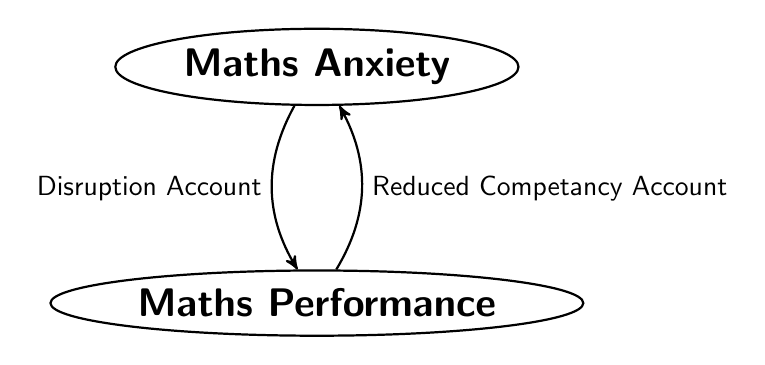
\begin{tikzpicture}[->,>=stealth',auto,node distance=3cm,thick,main node/.style={ellipse,draw,font=\sffamily\Large\bfseries}]
  	\node[main node] (a) {Maths Anxiety};
 	\node[main node] (b) [below of=a] {Maths Performance};

	\path	(a) edge[bend right] node [left] {Disruption Account} (b)
		(b) edge[bend right] node [right] {Reduced Competancy Account} (a);
\end{tikzpicture}
\end{document}
\caption{The Interpretation Account of 
Ramirez et al. (2018)
%\protect{\citeA{Ramirez2018}} 
for the maths anxiety-performance link showing how the Disruption Account and the Reduced Competency Account can be compatible.
\label{fig:ramirez}
}
\end{center}
\end{figure}

First, a brief summary of the two popular existing theories. The ``Disruption Account'', spearheaded by the work of Ashcraft et al., is focused on the concept of working memory \cite{Ashcraft2001, Ashcraft2007}. Specifically, Ashcraft et al. claim that anxiety takes up working memory capacity in a student's mind, which prevents them from using that working memory to complete maths tasks and in that way impacts on their performance in said tasks. In seeming contrast, the ``Reduced Competency Account'' proposes the opposite causality: that low maths ability leads to poor performance and affectively negative experiences of maths, which leads to an association between maths and negative affect to be formed in a students mind, i.e. causing maths anxiety to develop. There is a substantial body of work to support this hypothesis, including the landmark meta-analysis of \citeA{Hembree1990} and the longitudinal study of \citeA{Ma2004} which found that although past maths anxiety was correlated with future maths performance it was a small effect, while past maths performance had a strong effect on future maths anxiety.



\subsection*{Complexities in Finding Effective Interventions}

The models for the causation structure in the maths anxiety-performance connection presented above are of course broad oversimplifications of what is an incredibly complex and interconnected topic. They do however imply very different approaches for intervention. The ``Reduced Competency Account'' suggests interventions that boost maths performance and hence allow students to experience success in math should also help to reduce maths anxiety. The results of  \citeA{Supekar2015} seem to support this hypothesis as when students are given an intensive 8-week tutoring program to boost their maths skills, this is associated to a reduction in maths anxiety. The earlier work by \citeA{Faust1996} further supports via an anxiety-complexity effect in which low and high maths anxiety groups performed similarly on low complexity problems, but in high complexity problems the high anxiety groups performance was impacted. However, \citeA{Jansen2013} showed that it is not neccessarily as simple as these studies suggest --- they showed that when students experience success they attempt more problems and perform better but that when the confounding factors are modelled accurately enough it can be shown that the improved performance is almost completely predicted by the number of problems attempted, not their experience of success. Furthermore, \citeA{Jansen2013} showed that the level of maths anxiety was not affected in a significant way when experience of success was varied, which raises a lot of interesting but as yet unanswered questions. 
	
In contrast to the ``Reduced Compentency Account'', the ``Disruption Account'' implies that maths anxiety itself should be the target of interventions, and that if the maths anxiety is successfully reduced this will result in more free working memory and hence boost student performance. Following this line of reasoning, \citeA{Park2014} demonstrate a direct and successful attempt at this type of intervention where they used expressive writing exercises to guide students self-perceived narratives about their experiences with maths and reduce their maths anxiety. Notably the approach of \citeA{Park2014} is similar to successful approaches to the treatment of clinical anxiety disorders \cite{McNally2007, Becker2007,Foa2005}. Another approach drawn from the clinical psychology literature is that of reappraisal \cite{Jamieson2016}. In this approach stress is reconceptualised as a coping tool, a physiological response the purpose of which is to improve physical and mental performance in response to a challenge to be overcome. By reconceptualising stress in this productive way, rather than as a symptom of exposure to something to be feared and avoided, this approach does not neccessarily aim to directly reduce stress and anxiety levels in students, but instead allow them to perform despite the stress. This change in the perspective of stress is also very much in line with other parts of the literature discussing ``productive struggle'' \cite{Wang2015}, including some of the discussion of the ``Interpretation Account'' by \citeA{Ramirez2018}.

Intrinsic motivation has been shown to have an important mediating role in the relationship between Maths anxiety and performance \cite{Wang2015}, and serves as a crucial link in the ``productive struggle'' mindset. This reconceptualisation to a `productive struggle' model is not an isolated occurance in the literature. \citeA{Lin-Siegler2016} tells stories about the struggles experienced by famous scientists to students in an attempt to help normalise the concept of productive struggle in the context of a science classroom. \citeA{Hiebert2007} similarly provide a discussion on the importance of the ``productive struggle'' concept but specifically in a maths context.

One of the implications of the ``Interpretation Account'' proposed by \citeA{Ramirez2018}is that if an intervention targets only one causal direction in the cycle of \reffig{ramirez}, the cycle is likely to re-establish and negate any potential longterm effects. However the research of such longterm effects is very limited, and several authors have discussed the need for further research into this \cite{Pellicioni2016,Chang2016}. None-the-less, the limited literature that does exist discussing this seems to agree that the apporach most likely to be successful is one that targets both causal directions simultaneously, i.e. that focuses on both improving maths performance and reducing maths anxiety, simultaneously. This is very much in line with several of the other frameworks discussed in this work, not least of ll the curriculum-assessment diamong of \reffig{diamond} in which it is emphasised that while content is important, it is only equally as important as the learning experience. If students are not taught the required content they will not succeed, but if they are taught the required content and their experience of learning it is filled with anxiety and stress, they will also not succeed. The path to acheiving student success is clearly one in which both aspects are considered. 

%\subsection*{Instruments for Measuring Maths Anxiety}
%
%In order to track the effectiveness of these interventions, we will be collating assessment results as a measure of performance, but will also want to measure maths anxiety and maths affect/ self-concept. Significant work has been done over the years to develop psychometrics to measure maths anxiety, almost exclusively consisting of self-reporting surveys (with the exception of some more modern \gls{fmri} work, such as that of \citeA{Lyons2012}). We will use a recently developed scale: the \gls{mas-r} of \citeA{Bai2009}, which has been shown to be remarkably self consistent by incorporating both positive and negative affect items \cite{Bai2011}. It is short, easy to implement, and cheap in comparison to \gls{fmri} methods. In order to measure maths self-concept, \citeA{Jansen2013} modified the Perceived Competence Scale for Children of \citeA{Harter1982} to measure ``Math Competance''. The methodological process imployed by \citeA{Jansen2013} was quite rigorous and so we will use their instrument, or a minor modification thereof (we will do it in English), to measure maths self-concept.











\section{Self-Efficacy}

Much of the early research into self-efficacy has been structured based on the ``social cognitive theory'' of Bandura, so it seems appropriate to begin with a quote. \citeA[pg391]{Bandura1997} defines self-efficacy as 
\begin{quote}
``people’s judgement of their capabilities to organize and execute
courses of action required to attain designated types of performance''
\end{quote}


The connection between student's mathematical self-efficacy and their success in university preparatory mathematics courses has been well established in the literature \cite{Burton1987, Klinger2006, Klinger2011}. 

To quote \citeA{Johnson2016}:
\begin{quote}
``Self-efficacy
is vital among all students but particularly among adult learners as an individual’s
beliefs of self-capability has been shown to affect motivation, performance, achieve-
ment, effort, willingness to persist with a task, as well as the anxiety they experience
\cite{Bandura1997, Pajares1994, Pajares1996, Pajares1997, Pajares1999}. Woodley (1987) (cited in \cite{McGivney1996}) noted that the main personal
factors that contribute to dropout are: self-perception, being disorganised, not
having sufficient study skills and lacking in self-confidence. This suggests that an indi-
vidual’s self-efficacy plays a role in their decision with regard to dropping out.

\cite{Hackett1989} and \cite{Pajares1994} and Pajares and Miller (1995) also found that self-
efficacy can have an impact on career choice. In these studies, it was found that math-
ematical self-efficacy is a stronger predictor of students’ mathematical interest and
choice of degree programmes than either prior mathematical achievement or math-
ematical outcome expectations. Self-efficacy also influences how often mathematics
is used, as well as an individual’swillingness to pursue advancedwork in mathematics,
and even the choice of prospective occupations (Dutton and Dutton 1991). Engineers
Ireland (2010) highlight that this avoidance of mathematics, and mathematics-related
courses, at university will eventually prove detrimental when attempting to build a
knowledge economy. This point was also stressed decades before by \cite[pg34]{Hembree1990}
when he stated that ‘when otherwise capable students avoid the study of
mathematics, their options regarding careers are reduced, eroding the country’s
resource base in science and technology’.''
\end{quote}

 It is also well established that mathematical self-efficacy is strongly correlated to a combination of current knowledge/skills and current performance, with females and those who have not studied in a longer period of time generally having lower self-efficacy \cite{Carmichael2006, Carmichael2005}. In a group of so-called ``adult learners'', \citeA{Klinger2006} confirmed a result from several previous studies and showed that although the negative perceptions of mathematics widely held by the general population and demonstrated to negatively impact on mathematics performance where represented strongly on initial enrollment into a mathematics bridging course, that these negative perceptions changed dramatically during the course. The conclusion being that although yes, these negative perceptions of mathematics are highly predictive of performance, they can also be substantially influenced by early learning experiences, and should certainly not be thought of as fixed variables. In a later study, \citeA{Klinger2008} replicated a similar study but accross several diciplines of study and showed that arts/humanities had substantially lower mahtematical self-efficacy and more negative perceptions towards mathematics than the science students. Notably,  \citeA{Klinger2008} also showed a strong link between their quantitative results around mathemaical self-efficacy/ negative perceptions of mathematics and gender --- with female students scoring worse than males. All this research only further supports that weak mathematical skills cannot be addressed with content alone, but that the students negative preconceptions towards mathematics and poor mathematical self-efficacy views must also be addressed in order to support students on their way to success in a variety of fields of study, not only the study of mathematics. These results are all strongly in support of the \citeA{Ramirez2018} ``Interpretation Account'' framework shown in \reffig{ramirez} as well as the ``curriculum-diamond'' model shown in \reffig{diamond} in the sense that they imply a joint approach is required: simultaneously improving students knowledge/ skills and their self-efficacy/ affect towards mathematics. These two are so inextricably linked, that one cannot hope to successfully address one without also addressing the other. \cite{Taylor2006} used conversation theory framework to design an approach that was intended to simultaneously develop students' mathematical knowledge/ skills  and improve their mathematics self-efficacy/ confidence, which was shown to be effective. 

To summarise in the words of \citeA{Galligan2008}:
\begin{quote}
``... although attitudes and beliefs about mathematics are important for students
enrolled in bridging programs, the programs can change students' attitudes and
beliefs about mathematics as well as their achievement.''
\end{quote}












\section{Implications for Bridging Courses}

One of the primary roles of bridging courses is to facilitate students secondary-tertiary education transtition. Often the students enrolling in bridging courses will have either:\begin{itemize}
	\item Performed poorly in mathematics in secondary school, 
	\item Chosen to study mathematics at a intermediate or elementary level in secondary school, or
	\item Had a substantial time gap between completeing secondary school and engaging in tertiary education,
\end{itemize}
or some combination thereof. All of these possibilities will be associated with higher than average levels of mathematics anxiety, and negative preconceptions of mathematics. So, in this context, the question here is

\begin{quote}
How can a bridging course best support students through their transition into tertiary education?
\end{quote}

At a fundamental level, there are two key barriers that these students must overcome to be successful in their tertiary education:
\begin{itemize}
	\item Developing sufficient mathematics skills, capabilities, and knowledge. This can be addressed through content --- curriculum, and traditional teaching practices. 
	\item Overcoming/ changing negative perceptions/affect/anxiety towards mathematics. This is difficult to address, but there are a number of approaches suggested in the literature. 
\end{itemize}
One conclusion that is consistent with all the literature reviewed in this chapter, and is an implication of two of the major frameworks considered in this work: the curriculum-assessment diamond framework shown in \reffig{diamond}, and the interpretation account of shown in \reffig{ramirez}, is that these two key barriers must both be addressed simultaneously in order to have an effective and longlasting impact on student's success. 

Students having completed bridging courses have commented on the importance of this kind of combined approach. In the survey of \citeA{Gordon2013}, 
\begin{quote}
``students are aware of the value of the
bridging courses not only to ameliorate prior difficulties with mathemat-
ics and improve their approaches to learning mathematics but, less trans-
parently, as an important opportunity to facilitate their transition into
higher education, meet fellow students and help realise their potential.''
\end{quote}

Core to addressing the first of these two key barriers is the content, and what the appropriate content to teach in the bridging courses will be the focus of \refchap{curriculum}. In terms of how to best address the second these key barriers, there are a number of points on which there is broad agreement amongst the literature reviewed in this chapter, but there is a single message that draws together most of these points, which is to:
\begin{center}
	{\large SET CLEAR EXPECTATIONS.}
\end{center}
To give some examples of how this is featured in the literature, the ``rite-of-passage'' model of \citeA{Clark2008} suggests it is critical to set clear expectations around the new (tertiary) learning environment, as students are transitioning into a new and unfamiliar social environment/ community, it is critical to be explicit with them about the expectations in this new environment (i.e. independant learning, didactic lectures, etc.). The ``rite-of-passage'' model also suggests it is important that expectations be set for students about the difficulty of this transition beforehand (in the years prior to them making the transition to tertiary education) so that they come into the transition expecting it to be difficult and therefore being prepared for that difficulty. This perspective is further supported by the literature on how the perspective of viewing the process of learning mathematics (or learning in general) through the lens/  expectation of ``productive struggle'' particularly in the context of intervening to help maths anxious students \cite{Wang2015, Lin-Siegler2016, Hiebert2007, Carlson1999}.  Similarly, approaches taken from clinical psychology for the treatment of generalised anxiety disordershave been successful in helping maths anxious students, and reflect the same principles behind the concept of ``productive struggle''. Universities relaxing pre-requisites to ``assumed knowledge'' is a good (bad) example of \emph{not} setting clear expectations, and this impacting directly on students \cite{Gordon2015}. Some of these points are beyond the scope of this work, but there are also actions that can be taken from the perspective of teaching a bridging course to mitigate some of these concerns: even if students come into university without the expectation of it being a difficult culture-shock event and are not prepared, being clear and explicit with them about how it will be difficult, but that that is ok, can help. Similarly, changing university entry requirements is beyond the scope of this work, but even so when students come into the bridging courses with misconceptions such as ``mathematics is not important to being successful in science'', correcting these misconceptions can be very beneficial for them in terms of their success in pursuing their goals.

Additionally, although most of the reccomendations fall under ``set clear expectations'', some do not, these additional reccomendations include:
\begin{itemize}
	\item Helping students meet other students, make friends, and develop a social support network in their new environment is critical to supporting them to be successful, this is implied by the ``rite-of-passage'' framework of \cite{Clark2008}, but also by a swath of other literature \cite{Trotter2006, Peat2001, Leese2010, Gordon2013}.
	\item An emphasise on ``learning-to-learn'' programmes has been shown to be effective \cite{Zeegers2001}
\end{itemize}


Finally, there are some other important discussion points to be aware of, although no specific actionable reccomendations come from them:
\begin{itemize}
	\item Success in secondary school mathematics is highly predictive of success and even participation in tertiary mathematics education. This predictive effect is larger tha n the effect of any bridging course on retention and success in tertirary eduction \cite{Kajander2005, Nicholas2015b}. This is important to be aware of, but unfortunately falls outside of the scope of a bridging course to address. Instead, we have to rely on secondary school educators to continue working to improve this.
	\item Negative community perceptions of mathematics influence rates of maths anxiety, engagement and ultimately success in mathematics educations of our students \cite{King2015, Gordon2013, Clark2008}. Again, negative community perceptions is (somewhat) beyond the scope of a bridging course to address but it is critical to be aware of the impact it has, and to be fair it does fall on all mathematicians but even more so non-mathematician mathematically skilled people and educators (including those teaching a bridging course) to gradually create the social change needed to adjust such widespread community perceptions. Broad cultural change is somewhat beyond the scope of this work, however.
\end{itemize}







%
%\newpage
%
%\section{Temporary Section: TODO List}
%
%TODO List (Papers to read in more detail, and incorporate into discussion):
%\begin{itemize}
%	\item 
%	\item \cite{Irwin2018} Talks about the importance of alternate avenues to access education. --- read and summarise again.
%	\item Some of the books I found would be good to read more thoroughly too, \cite{Volmink1994} for example, and/or \cite{McGivney1996} for example.
%	\item Quote from \cite{Galligan2008} covering some concepts that would be nice to incorporate into the discussion somewhere:
%		\begin{quote}
%		\citeA{Miller2006}, in a significant long term analysis of two large bridging
%		courses and one individual bridging program in New Zealand, used quantitative
%		and qualitative measures to compare students' reactions. These multiple strands of
%		evidence provided a complex overall picture of three largely successful teaching
%		approaches. A one-to-one supervised course focused on understanding fear of
%		mathematics and early mathematics experiences. The course empowered the
%		student who came to believe that mathematics was a creative and enjoyable
%		process. A second course (100 students) focused on the mathematization of
%		realistic situations. Here, students came to regard mathematics as useful,
%		interesting, and relevant to real life. The third course (100 students) was a carefully
%		structured re-introduction of mathematics. The students appreciated the course and
%		were pleased that they could now do mathematics that they could not do in schqol.
%		Students in all programs were highly motivated, mature, and had not seen formal
%		mathematics for some years. One surprising result from the study was that if
%		students were unsuccessful they were, in fact, worse otT than before, and often
%		confused. A significant component of the study was the focus placed on dealing
%		with students' mathematics anxiety or fear. Quantitative measures and qualitative
%		descriptors indicated a decrease in mathematics anxiety throughout the duration of
%		the three programs, and in the larger courses this correlated with achievement.
%		Beliefs about mathematics in general, however, did not necessarily change,
%		although students in the larger courses did see the practical nature of mathematics.
%		\end{quote}
%
%	\item Student wellbeing is a research interest, with high strain in the first semester at uni \cite{Bewick2010}
%\end{itemize}



\cleardoublepage
\chapter{Curriculum Mapping}
\label{chap:curriculum}

%TODO: I should add a comment here somewhere about how initially I will be simply comparing content, but that by the end of this chapter I will also consider requirements/ expectations of the bridging course RE MathsStart aliging roughly to year 11 material and MathsTrack covering Maths Methods but not neccessarily Maths Specialist, etc.

One of the important roles of university mathematics bridging courses (such as MathsStart and MathsTrack) is to fill the content knowledge gap for students who  wish to commence study that has some required knowledge and skills in mathematics, but either did not complete mathematics to a sufficiently high level in highschool, or completed it long enough ago that they need to re-learn the skills. Ultimately, the content of such bridging courses needs to align with the ``Industry Standards'' or ``Standards of Performance'' and in particular the ``Curriculum Objective'' of the curriculum assessment diamond model (\reffig{diamond}). 

There are two key perspectives that can be taken on what the ``Curriculum Objective'' of a mathematics bridging course is: the knowledge required for the future (tertiary) study the students are going to engage in, and knowledge expected from highschool graduates. As we will come to see, these two angles or perspectives can be quite dramatically different. From the perspective of knowledge expected from highschool graduates, in Australia the \gls{ac} serves as a good guide, but even so the exact content knowledge expected of students having completed highschool in Australia varies for a number of reasons:
\begin{itemize}
	\item To begin with, the \gls{ac} specifies four levels of mathematics: essential mathematics, general mathematics, mathematical methods, and specialist mathematics. Our focus will be on the higher two of these: mathematical methods and specialist mathematics, as these are the ones targetted at university entry into mathematics-intensive courses. 
	\item Different states within Australia teach different curriculums, with varying degrees of alignment to the \gls{ac}. In South Australia the primary curriculum taught in senior secondary school is \gls{sace}, and so we will focus on that.
	\item Occasionally, students will do the bridging course and then travel internationally to study in which case the expectations placed on them will be based on an entirely different curriculum. This is comparatively rare, but also the modern international education system has a remarkable level of homogeniety partially as a carry-over consequence of the western colonial era \cite{Mohandas2003}. Regardless, it is beyond the scope of this work to consider alignment of content to highschool curriculums internationally, although this would make for interesting future research.
\end{itemize}
The other perspective is of course also important, but also far more difficult to address: the knowledge required for entry level university mathematics courses. This will vary hugely from course to course: a entry level calculus course will require very different knowledge than an entry level statistics course, for example. Even within one discipline of mathematics, different universities will have very different expectations of entry level students: in particular, South Australian universities will often structure their entry level mathematics courses to align with \gls{sace} even though not all their students have completed \gls{sace}, because of the majority who have it is still useful for them to do so. For example, the University of Adeliade re-structured it's first year mathematics courses in 2018 to match changes in \gls{sace}. Similarly, universities interstate will often structure their entry level courses to align with their local senior highschool curriculum. That is only within dedicated mathematics courses, other courses that also require mathematics knowledge and skills, such as engineering, psychology, health science, and medicine will all have their own requirements. Bridging courses will enroll students aiming to study a wide variety of such topics, and even more broadly also to go into non-university further study (notably pilot training in the defence force, for example), which have different requirements again.

This places a difficult tension on mathematics bridging courses as to what content to teach. Although many of the students enrolling in the mathematics bridging courses at the \gls{uofa} do so with the intention to begin study at the \gls{uofa} (and hence might benefit from \gls{sace} structured content), many do not. Even amongst those that do, some may end up going to a different university interstate or even overseas --- plans change. So it is important to try and maintain some connection to a broader set of knowledge expected in general and not neccessarily remain laser focussed on the requirements of the particular university courses most students are going to be attempting. This is one of the reasons why the \gls{ac} is a useful construct as even though some states do not align to the \gls{ac} as well as others, it still forms a guiding structure at a national level and individually considering the curriculum taught in each state is beyond the scope of this work. Tailoring the content of the bridging courses more narrowly to target entry into particular disciplines (say calculus/ matrix algebra/ statistics for example) could potentially still be of interest down the line, but is likely to be unrealistic with the current resources available to the \gls{uofa} \gls{mlc}.

Because of the difficulty of aligning the content to the future requirements of students due to their variety of different directions and needs, and considering that the majority (over half) of students enrolling in MathsStart and MathsTrack plan on enrolling in tertiary study at the \gls{uofa}, the focus of this curriculum mapping will be on aligning the content of the bridging courses to the \gls{sace} curriculum. That said, the alignment of the \gls{sace} curriculum to the \gls{ac} will also be considered, in order to give some idea of the national alignment (and it turns out the \gls{ac} is very closely aligned to the \gls{sace} curriculum). Now that said, the different directions students are going is still very important to consider, and although a direct alignment to the plethora of options students pursue is not realistic, the needs of the most common of these options will be incorporated into the discussion surrounding the curriculum alignment presented in this chapter. Even if direct alignment to these needs cannot be acheived, it is none-the-less important to be aware of these needs, as these are critical to students future success, and while it might not be realistic to tailor the content of the bridging courses to each of these contexts, differentiation can still be acheived through an awareness of these needs and individual interactions with students each of which will often have a particular future direction in mind.

This chapter will be structured as follows. First, in \refsec{content}, some notation will be introduced and the content of each of the three curriculums that will be systematically reviewed:
\begin{itemize}
	\item The \gls{ac} senior mathematics subjects mathematical methods and specialist mathematics,
	\item The \gls{sace} curriculum stage 1 mathematics, stage 2 mathematical methods, and stage 2 specialist mathematics,
	\item The University of Adelaide's bridging courses: MathsStart, and MathsTrack.
\end{itemize}
Note that the alignment done here is entirely on the content of these curriculums, nothing else. The focus of this chapter is entirely on content. The alignment between the content in these curriculums will be considered in \refsec{mapping} (see \reffig{mapping}), and alignments/ misalignments discussed. Finally, the discussion throughout around alignment and gaps between the content of these curriculums and courses will be summarised, explanations and reasons for these discrepancies discussed, and potential modifications to content suggested. 

Beyond that, this chapter will also briefly discuss the alignment of these bridging courses to first year university mathematics courses and bridging courses offered by other universities in Australia, and discuss the relationship between the gaps in alignment between the \gls{ac}/\gls{sace} and the bridging courses and the requirements of these first year university courses. 



\section{Content}
\label{sec:content}

The curriculum alignment in this chapter is presented at two levels of detail --- the topic level, and the key concept level. The terms ``topic'' and ``key concept'' are reserved in the context of this discussion to specifically refer to these levels of detail. The content of each of the senior highschool curriculums, as well as the university bridging courses, is broken down into topics, and each topic can be summarised as covering a number of key concepts. In \refsec{mapping}, the alignment between these curriculums and bridging courses will be considered thoroughly at both a topic-level, and to the finer detail of particular key concepts. Although the key concept alignment is in essence the core of the work, as this is what allows for concrete changes to be made and content to be planned, the purpose of the topic level comparison is to help structure the overall alignment and discussion. 

\subsection{Notation}

In order to provide a useful curriculum-wide topic-level alignment to structure our thinking, it is important to be able to present this alignment in a comprehensible form that can be viewed on a single page. In order to acheive this, the topic-level description (identification of topics) needs to be summarised concisely enough. This is acheived in Figures~\ref{fig:mapping} and \ref{fig:mappingByTopic}, by identifying each topic with an abbreviated code. These abbreviated codes are presented in \reftab{notation} and will be used for the remainder of this chapter to help refer to and identify topics. Each topic in each of the curriculums being considered is assigned a unique identifying code in \reftab{notation}, and the curriculum (and subject within it) can be easily seen from the structure of the code.

\begin{table}[h]
\caption{Abbreviated codes for topics within the \gls{ac} and \gls{sace} senior mathematics subjects: Mathematical Methods nd Specialist Mathematics, as well as the Unviersity of Adelaides bridging courses: MathsStart and MathsTrack. Square brackets ([]) are used to indicate numeric values that can vary. \label{tab:notation}}
\begin{tabular}{ll}
Code & Meaning \\ \hline
 & \\
MMu[\#1]t[\#2] & \gls{ac} Senior Mathematical Methods Unit [\#1], Topic [\#2] \\
MMu[\#1]t[\#2] & \gls{ac} Senior Specialist Mathematics Unit [\#1], Topic [\#2] \\
 & \\
S1M[\#] & \gls{sace} Stage 1 Mathematics, Topic [\#] \\
S2MM[\#] & \gls{sace} Stage 2 Mathematical Methods, Topic [\#] \\
S2SM[\#] & \gls{sace} Stage 2 Specialist Mathematics, Topic [\#] \\
 & \\
MS[\#] & Maths Start, Topic (Booklet) [\#] \\
MT[\#] & Maths Track, Topic (Booklet) [\#]
\end{tabular}
\end{table}

\subsection{Key Concepts}

\refapp{concepts} provides a description of each topic in each of the curriculums considered here: the \gls{ac} Mathematical Methods and Specialist Mathematics, \gls{sace} stage 1 mathematics, stage 2 mathematical methods and stage 2 specialist mathematics, and the \gls{uofa} MathsStart and MathsTrack programs. For brevity, the codes from \reftab{notation} are used to identify each topic. The name of each topic is given in bold, followed by a list of the key concepts covered in that topic seperated by commas. These are discussed at length for the remainder of this chapter, and the table presented in \refapp{concepts} is intended to be used as reference material while reading the content of this chapter.

Some notes on the way the key concepts are summarised:
\begin{itemize}
	\item The key concepts listed for each topic are intended for a reader deeply familiar with the content, and as such it is heavily condensed and uses standard mathematical notation and terminology without the usually appropriate rigorous definitions. 
	\item Concepts relating to "interpretation" and application in a general sense are ommited from the key concepts of a topic. The assumption is that to the intended readers, these should go without saying. For example, in S1M2 the key concept "Quadratic Equations in Vertex and Factorised Form" is included, but this implies a variety of auxillary knowledge which is not explicity included in the key concept summary: the interpretation of roots and vertices, deducing vertices and roots from the equation of a quadratic, or deducing the equation of a quadratic given these bits of information, etc. These are skills directly and universally associated to the key concept, and it is assumed that an experienced mathematics educator (which is the intended audience for this text) should be able to easily deduce such surrounding associated skills from the key concepts listed. 
\end{itemize}
These restrictions in the key concept summaries are neccessary in order to be able to present this curriculum alignment concisely enough that it can be useful. The curriculum documents used to generate these summaries contain all the additional detail if required, but the purpose of this work is to align the content in those documents to identify gaps and mis-alignments, and as such it is beneficial to be as concise and dense as possible both to make the alignment a tractable problem and also to make the discussion thereof comprehensible. That said, it is a delicate balance between being broad and vague in order to be able to present the entire curriculum mapping within a single frame of view, and yet still be granular enough so that specific content is clear and explicity and useful actionable reccomendations can be made. It is this tension that led to the development of the methodology which split the two levels of detail: 
\begin{itemize}
	\item The topic level description is intended to give the broad strokes, to show the entire mapping in a single frame of view (a page, in this case). It is also intended to be reference material for the following more detailed discussion, to aid the reader in structuring the information contained in the more detialed discussion and place each peice of information into where it belongs in the bigger picture. Being able to structure the detailed discussion into this larger concept is critical for being able to reach broad overall conclusions.
	\item The key concept level is what comprises the bulk of the discussion, and this is intended to be the grandular level at which content is presented specifically enough that reccomended actions can be understood explicitly and implemented easily. Note that although the key concept level is much more granular than the topic level discussion, it is still intended as a summary and does not include every single detail of the content, as discussed above.
\end{itemize}



\subsection{Curriculum Structure}
\label{sec:structure}

\subsubsection{The \gls{ac}}

The \gls{ac} is separated into it's F-10 curriculum, and senior secondary curriculum. In this work we are only concerned with the senior secondary curriculum. The senior secondary \gls{ac} for mathematics is split into four subjects, corresponding to different ``levels'' of mathematics: Essential Mathemaics, General Mathematics, Mathematical Methods, and Specialist Mathematics. In this work we are concerned only with Mathematical Methods and Specialist Mathematics, and will be considering the mathematical content of these subjects not any other aspects (such as cross-curricular priorities, for example). Importantly, the senior secondary \gls{ac} does not make any distinction between years 11 and 12 (typically the final year of highschool in Australia). So the senior secondary \gls{ac} subject ``Mathematical Methods'' for example, covers content that is in practice taught accross both years 11 and 12. Each of the two subjects we are concerned with in this work, Mathematical Methods and Specialist Mathematics, are split into four ``units'' of content, and each of these units is split into three topics, for a total of 12 topics per subject, and a total of 24 topics that we will consider from the \gls{ac}. At no point do we consider the unit structure of the \gls{ac}, partly because it does not have any analog in the other curriculums we are aligning too, but mostly because it does not give a useful level of detail for our purposes.

\subsubsection{\gls{sace}}

\gls{sace}, in comparison to the \gls{ac}, does distinguish between year 11 and year 12 content, although to allow for some alternative senior highschool teaching structures they have a different naming convention, calling them stage 1 and stage 2 respectively. In the majority of mainstream cases in Australia, \gls{sace} stage 1 will correspond to year 11, and \gls{sace} stage 2 will correspond to year 12. To further complicate matters, stage 1 \gls{sace} has only three levels of mathematics: Essential Mathematics, General Mathematics, and Mathematics, while stage 2 \gls{sace} has four: Essential Mathematics, General Mathemaitcs, Mathematical Methods, and Specialist Mathematics. In this work we will only be concerned with \gls{sace} stage 1 Mathematics, stage 2 Mathematical Methods, and stage 2 Specialist Mathematics. \gls{sace} stage 1 Mathematics is broken down into 12 topics, while stage 2 Mathematical Methods and Specialist Mathematics are broken down into 6 topics each. This makes for a total of 24 topics from senior highschool \gls{sace} mathematics subjects that we will be considering in the curriculum alignment presented in this chapter.

\subsubsection{\gls{uofa} Bridging Courses}

The \gls{uofa} offers two bridging courses through their \gls{mlc}: MathsStart and MathsTrack. These are both taught through a series of booklets which conveniently each contain roughly on ``topic'' worth of content, and so these booklets will be used as the topic-level structure of these courses. Both courses are currently structured into 8 topics (booklets) each, although MathsTrack used to have 9, and the fifth was removed some time ago, so the numbering of the MathsTrack topics have a gap (they are numbered 1, 2, 3, 4, 6, 7, 8, 9). So there are a total of 16 topics (booklets) accross both bridging courses that will be considered in the curriculum alignment presented in this chapter.

\subsubsection{Topic Grouping}

In order to help structure the discussion to follow, it will be useful to think about one broader level of detail, which will loosely be refered to as ``content areas''. From a very low level of detail perspective, the topics in each of the curriculums being considered can be grouped into the following five broad content areas:
\begin{itemize}
	\item Functions and Graphs, 
	\item Calculus, 
	\item Geometry and Linear Algebra, 
	\item (Complex) Numbers, and 
	\item Probability and Statistics	
\end{itemize}
There is also some nested hierachicial structures within these content areas that are useful to understand. For example, both ``Functions and Graphs'' and ``Calculus'' can be further separated into three sub-areas, corresponding to different categories of functions. Specifically: 
\begin{itemize}
	\item Linear, Polynomial, and Rational Functions,
	\item Exponential and Logarithmic Functions, and
	\item Trigonometric Functions.
\end{itemize} 
``Calculus'' is naturally divided into differentiation and integration, ``Probability and Statistics'' can be divided into probability and statistics as seperate content sub-areas, although more commonly is divided into discrete and continuous random variables. Geometry and Linear Algebra covers perhaps the widest variety of topics, from vectors to matrices to systems of equations as well as more traditional geometry topics such as circle theorems. 

The two areas (``Functions and Graphs'' and ``Calculus'') are also often taught together, with new categories of functions being introduced/ revised together with concepts around how to do calculus with these functions, so this particular pair of content areas are very closely linked. Although there are some notable connections between the other content areas, such as for example: 
\begin{itemize}
	\item Complex numbers providing a method for finding roots to polynomials that could not otherwise be found,
	\item Applying calculus to parameterised vector equations, 
	\item Integration being used to understand probabilities as areas under distribution functions,
\end{itemize}
Broadly speaking they stand comparatively apart from each other, particularly Probabilty and Statistics. 

This broad content area grouping of topics covers almost all of the content in all the curriculums considered here. The only notable exceptions being MMu2t2 from the \gls{ac} and S1M7 from \gls{sace} both covering primarily sequences (geometric and arithmetic) as recurrance relations, and S2SM1 from the \gls{sace} covering inductive proof, neither of which fit neatly into any of the content areas above. With that having been clarified, these content areas will be used to help structure the discussion for the remainder of this chapter.

%\subsection{\gls{ac} Mathematical Methods and Specialist Mathematics}
%
% \gls{ac} has four levels of mathmatics, including also essential and general mathematics. Mathematical Methods and Specialist Mathematics are the two highest level mathematics, intended (partly) for preparation to university entry. Broadly speaking, the content of these two subjects can be grouped into several areas:
%\begin{itemize}
%	\item Functions and Graphs, which is broken up primarily into families of functions, with some extra concepts thown into some generalist topics:
%		\begin{itemize}	
%			\item Polynomials and Rational Functions (MMu1t1, SMu3t2),
%			\item Exponentials and Logarithms (MMu2t1, MMu2t2, MMu4t1)
%			\item Trigonometric Functions (MMu1t2, SMu2t1)
%		\end{itemize}
%	\item Calculus, which is largely structured similarly to the Functions and Graphs: breaking it up by the type of function you are doing calculus on, splitting up differentiation from integration, and throwing in rules of differentiation and approaches to integration with a few extra concepts along the way (MMu2t3, MMu3t1, MMu3t2, SMu4t1, SM4t2).
%	\item Geometry and Linear Algebra: Mostly vectors, with some matrices, systems of equations, and even circle theorems. This is the topic in which the concept of proof is primarily attempted to be introduced, and perhaps that is the reason why it is entirely contained within the Specialist Mathematics curriculum (SMu1t2, SMu1t3, SMu2t2, SMu3t3),
%	\item Complex Numbers, as well as rational/ irrational numbers, etc. (SMu2t3, SMu3t1), and finally
%	\item Probability and Statistics, with some combinatorics thrown in for good measure (MMu1t3, MMu3t3, MMu4t2, MMu4t3, SMu1t1, SMu4t3)
%\end{itemize}
%Although there are a couple of topics (MMu2t2 for example) which although they relate to these broader areas, also contain a substantial amount of other content.
%
%More detailed discussion of the specific key concepts of interest will follow in \refsec{mapping} as a natural part of comparisons between curriculums, as that is where the specifics will be important. These sections are intended to give a broader overview of the structure of the content in these curriculums
%
%\subsection{\gls{sace} Stage 1 Mathematics, Stage 2 Mathematical Methods and Specialist Mathematics}
%
%\gls{sace} follows the \gls{ac} fairly well at a broad level (although there are differences in the details, which will be discussed in \refsec{mapping}. Broadly though the topics in the three \gls{sace} subjects here, although split into three subjects instead of two, can be broadly grouped into areas much the same as the \gls{ac}:
%\begin{itemize}
%	\item Functions and Graphs, which is broken roughy as:
%		\begin{itemize}	
%			\item General Concepts (S1M1, S2SM3),
%			\item Polynomials and Rational Functions (S1M2, S2SM3),
%			\item Exponentials and Logarithms (S1M5, S2MM4, S1M7)
%			\item Trigonometric Functions (S1M3, S1M10)
%		\end{itemize}
%	\item Calculus, which similarly split up by the type of function you are doing calculus on, differentiation vs integration, and throwing in rules of differentiation and approaches to integration with a few extra concepts along the way (S1M6, S2MM1, S2MM3, S2MM4, S2SM5, S2SM6).
%	\item Geometry and Linear Algebra: Mostly vectors, with some matrices, systems of equations, and even circle theorems. This is the topic in which the concept of proof is primarily attempted to be introduced, and perhaps that is the reason why it is entirely contained within the Specialist Mathematics curriculum (S1M8, S1M9, S1M11, S2SM4),
%	\item Complex Numbers, as well as rational/ irrational numbers, etc. (S1M12, S2SM2), and finally
%	\item Probability and Statistics, with some combinatorics thrown in for good measure is included almost exclusively in Stage 2 Mathematical Methods (S1M4, S2MM2, S2MM5, S2MM6)
%\end{itemize}
%Although there are a couple of topics (S1M7,for example --- very similarly to MMu2t2) which although they relate to these broader areas, also contain a substantial amount of other content. This grouping also leaves one topic out in the \gls{sace} context: S2SM1 which is essentially just the concept of mathematical induction.
%
%
%
%\subsection{MathsStart and MathsTrack}
%
%MathsStart can be seen as essentially an introduction to functions, MathsTrack then takes this, and extends it primarily to calculus, taking a little detour along the way to cover some vector and matrix geometry/ systems of linear equations concepts. So broadly grouping the topics in a way analogous to above:
%\begin{itemize}
%	\item Functions and Graphs, roughly broken up into:
%		\begin{itemize}
%			\item General Concepts (MS1, MS2),
%			\item Polynomials and Rational Functions (MS3, MS4, MT1),
%			\item Exponentials and Logarithms (MS7, MS8), and 
%			\item Trigonometry (MS5, MS6)
%		\end{itemize}
%	\item Calculus, similarly first introducing differentiation on polynomials with various other general concepts (MT6, MT7) and then exponentials and logarithms (MT8) and finally also integration (MT9).
%	\item Geometry and Linear Algebra (MT2, MT3, MT4).
%\end{itemize}
%
%Note the missing topic 5 in MathsTrack, this used to be part of the course some time ago but is currently no longer included in the content of the course, and so is not included here.








\section{Curriculum Mapping}
\label{sec:mapping}

\reffig{mapping} shows the topic-level alignment between the \gls{ac}, \gls{sace}, and bridging courses, organised by subject/ course. Each node (ellipse) in \reffig{mapping} corresponds to a topic, and is identified by the abbreviated code as per \reftab{notation}. What ``organised by subject/ course'' means in this context is that while the curriculla (the \gls{ac}, \gls{sace}, and the \gls{uofa} bridging courses) are arranged as columns in \reffig{mapping}, within each of these columns topics are grouped by subject. So for example in the \gls{ac} column topics are grouped into Mathematical Methods topics, and then Specialist Mathematics topics.

\clearpage

\pagestyle{empty}

\begin{figure}[p]
\begin{center}
\input{./figures/mapping}
\caption{Curriculum Mapping by Subject/ Course\label{fig:mapping}}
\end{center}
\end{figure}

\begin{figure}[p]
\begin{center}
% TiKz
\documentclass[tikz, 12pt]{standalone}
\usetikzlibrary{positioning}
\usetikzlibrary{shapes}

% Math
\usepackage{amsfonts}
\usepackage{amsmath}

% CMU sans serif font.
\usepackage[T1]{fontenc}
\renewcommand*\familydefault{\sfdefault}

\begin{document}
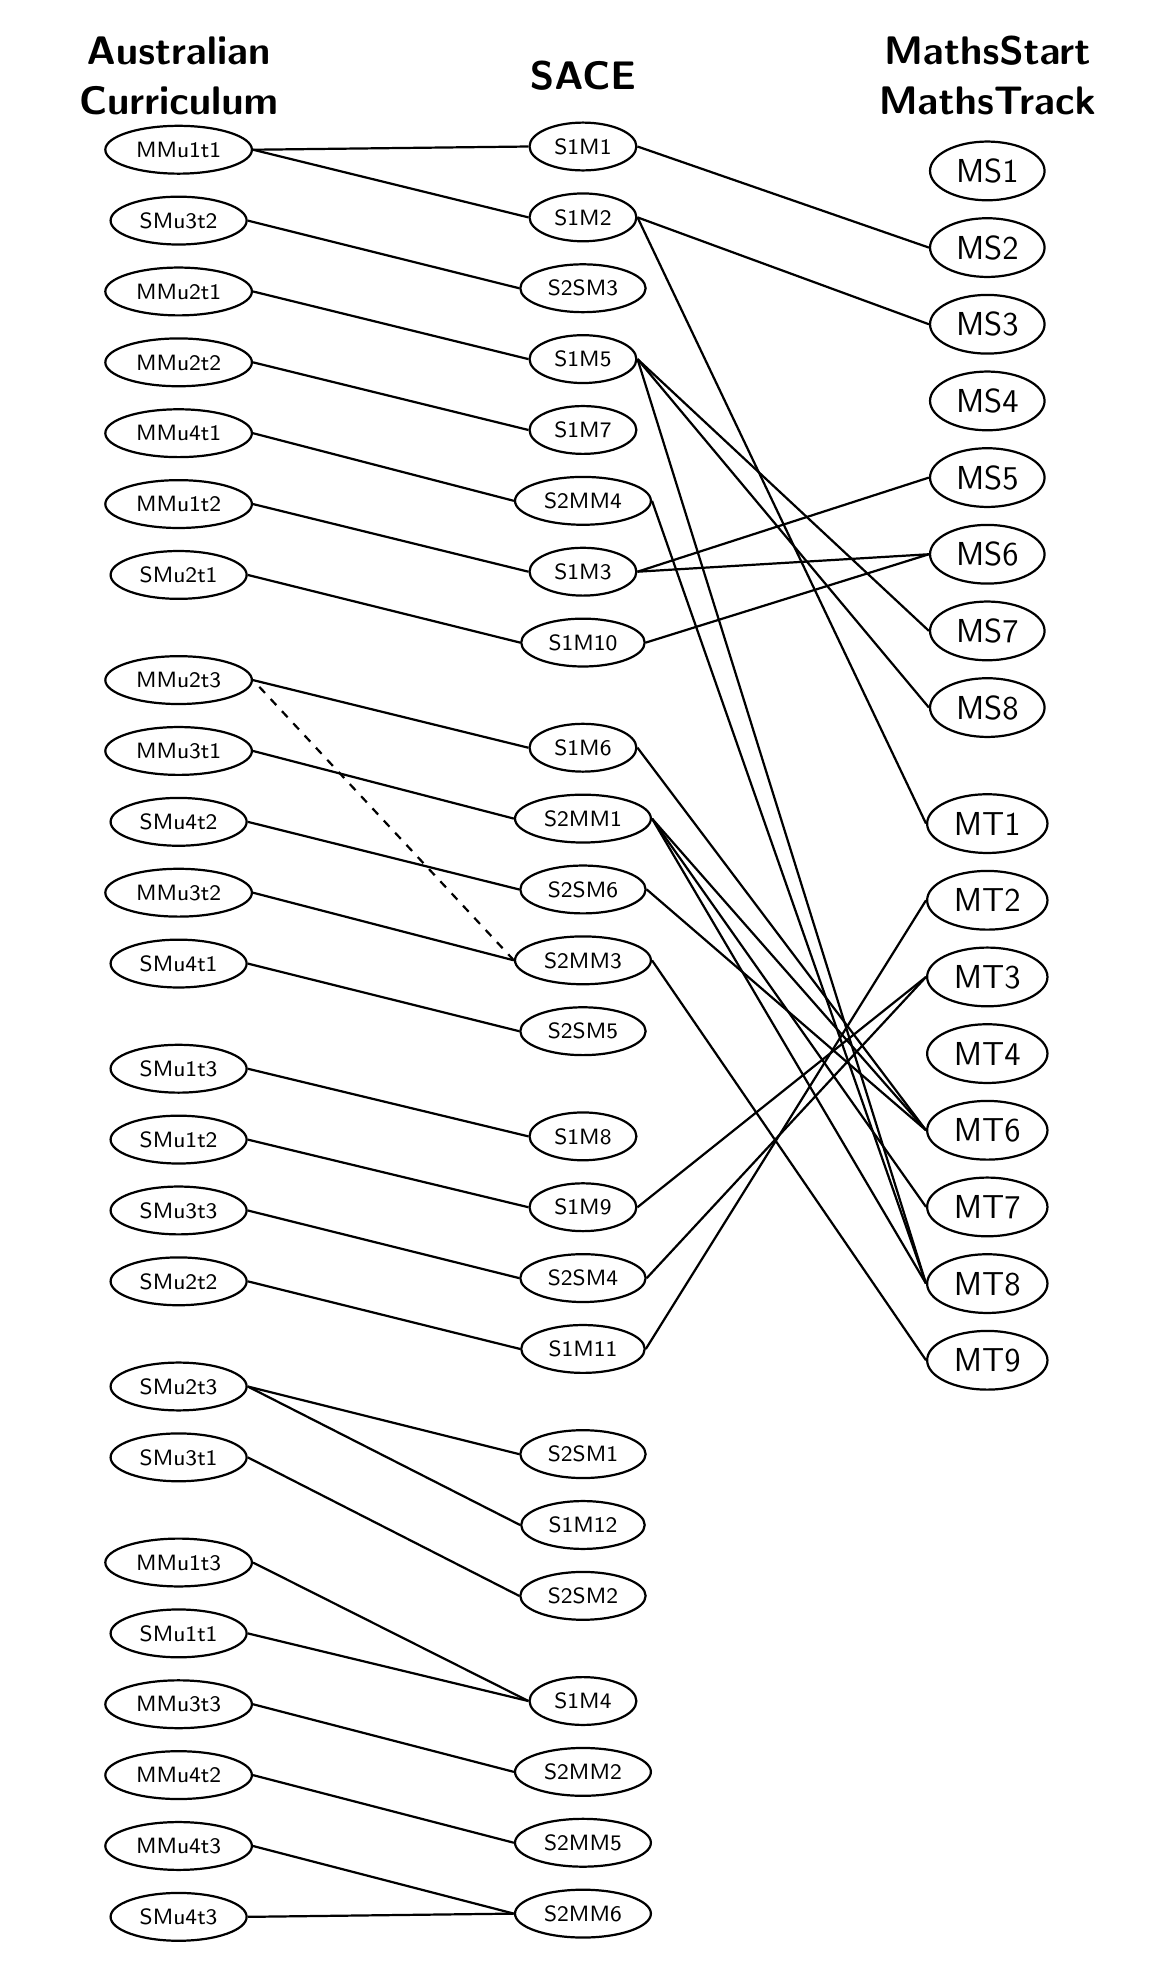
\begin{tikzpicture}[node distance=0.9cm,thick,topic node/.style={ellipse,draw,font=\footnotesize},unit node/.style={ellipse,draw,font=\large}]

	% MathsStart
	\node[font=\Large\bfseries, text width = 3.6cm, align=center] (ms) {MathsStart MathsTrack};
  	\node[unit node] (ms1) [below=0.2cm of ms] {MS1};
  	\node[unit node] (ms2) [below=0.2cm of ms1] {MS2};
  	\node[unit node] (ms3) [below=0.2cm of ms2] {MS3};
  	\node[unit node] (ms4) [below=0.2cm of ms3] {MS4};
  	\node[unit node] (ms5) [below=0.2cm of ms4] {MS5};
  	\node[unit node] (ms6) [below=0.2cm of ms5] {MS6};
  	\node[unit node] (ms7) [below=0.2cm of ms6] {MS7};
  	\node[unit node] (ms8) [below=0.2cm of ms7] {MS8};
%  	\node[unit node] (ms1) [below=0.2cm of ms] {Functions};
%  	\node[unit node] (ms2) [below=0.2cm of ms1] {Linear};
%  	\node[unit node] (ms3) [below=0.2cm of ms2] {Quadratic};
%  	\node[unit node] (ms4) [below=0.2cm of ms3] {Rational};
%  	\node[unit node] (ms5) [below=0.2cm of ms4] {Trigonometry I};
%  	\node[unit node] (ms6) [below=0.2cm of ms5] {Trigonometry II};
%  	\node[unit node] (ms7) [below=0.2cm of ms6] {Exponential};
%  	\node[unit node] (ms8) [below=0.2cm of ms7] {Logarithm};

	% MathsTrack
  	\node[unit node] (mt1) [below=0.7cm of ms8] {MT1};
  	\node[unit node] (mt2) [below=0.2cm of mt1] {MT2};
  	\node[unit node] (mt3) [below=0.2cm of mt2] {MT3};
  	\node[unit node] (mt4) [below=0.2cm of mt3] {MT4};
  	\node[unit node] (mt6) [below=0.2cm of mt4] {MT6};
  	\node[unit node] (mt7) [below=0.2cm of mt6] {MT7};
  	\node[unit node] (mt8) [below=0.2cm of mt7] {MT8};
  	\node[unit node] (mt9) [below=0.2cm of mt8] {MT9};
%  	\node[unit node] (mt1) [below=0.8cm of ms8] {Polynomials};
%  	\node[unit node] (mt2) [below=0.2cm of mt1] {Matrices};
%  	\node[unit node] (mt3) [below=0.2cm of mt2] {Vectors};
%  	\node[unit node] (mt4) [below=0.2cm of mt3] {Systems of Eqns};
%  	\node[unit node] (mt6) [below=0.2cm of mt4] {Differentiation};
%  	\node[unit node] (mt7) [below=0.2cm of mt6] {Differentiation Apps};
%  	\node[unit node] (mt8) [below=0.2cm of mt7] {Exp and Log};
%  	\node[unit node] (mt9) [below=0.2cm of mt8] {Integration};
  	
	% SACE
	\node[font=\Large\bfseries] (sace) [left=2.4cm of ms] {SACE};
	% Functions and Graphs
  	\node[topic node] (ss1m1) [below of=sace] {S1M1};
  	\node[topic node] (ss1m2) [below of=ss1m1] {S1M2};
  	\node[topic node] (ss2sm3) [below of=ss1m2] {S2SM3};
  	\node[topic node] (ss1m5) [below of=ss2sm3] {S1M5};
  	\node[topic node] (ss1m7) [below of=ss1m5] {S1M7};
  	\node[topic node] (ss2mm4) [below of=ss1m7] {S2MM4};
  	\node[topic node] (ss1m3) [below of=ss2mm4] {S1M3};
  	\node[topic node] (ss1m10) [below of=ss1m3] {S1M10};
	% Calculus
  	\node[topic node] (ss1m6) [below=0.7cm of ss1m10] {S1M6};
  	\node[topic node] (ss2mm1) [below of=ss1m6] {S2MM1};
  	\node[topic node] (ss2sm6) [below of=ss2mm1] {S2SM6};  	
  	\node[topic node] (ss2mm3) [below of=ss2sm6] {S2MM3};
  	\node[topic node] (ss2sm5) [below of=ss2mm3] {S2SM5};
	% Geometry and Linear Algebra
  	\node[topic node] (ss1m8) [below=0.7cm of ss2sm5] {S1M8};
	\node[topic node] (ss1m9) [below of=ss1m8] {S1M9};
  	\node[topic node] (ss2sm4) [below of=ss1m9] {S2SM4};
  	\node[topic node] (ss1m11) [below of=ss2sm4] {S1M11};
  	% Complex Numbers
  	\node[topic node] (ss2sm1) [below=0.7cm of ss1m11] {S2SM1};
  	\node[topic node] (ss1m12) [below of=ss2sm1] {S1M12};
  	\node[topic node] (ss2sm2) [below of=ss1m12] {S2SM2};
	% Probability and Statistics	
  	\node[topic node] (ss1m4) [below=0.7cm of ss2sm2] {S1M4};
  	\node[topic node] (ss2mm2) [below of=ss1m4] {S2MM2}; 	
  	\node[topic node] (ss2mm5) [below of=ss2mm2] {S2MM5};
  	\node[topic node] (ss2mm6) [below of=ss2mm5] {S2MM6};
  	
  	
	% Australian Curriculum
	\node[font=\Large\bfseries, text width = 3.6cm, align=center] (ac) [left=2.4cm of sace] {Australian Curriculum};
	% Functions and Graphs
  	\node[topic node] (acmmmu1t1) [below=0cm of ac] {MMu1t1};
  	\node[topic node] (acmsmu3t2) [below of=acmmmu1t1] {SMu3t2};
  	\node[topic node] (acmmmu2t1) [below of=acmsmu3t2] {MMu2t1};
  	\node[topic node] (acmmmu2t2) [below of=acmmmu2t1] {MMu2t2};
  	\node[topic node] (acmmmu4t1) [below of=acmmmu2t2] {MMu4t1};
  	\node[topic node] (acmmmu1t2) [below of=acmmmu4t1] {MMu1t2};
  	\node[topic node] (acmsmu2t1) [below of=acmmmu1t2] {SMu2t1};
	% Calculus
  	\node[topic node] (acmmmu2t3) [below=0.7cm of acmsmu2t1] {MMu2t3};
  	\node[topic node] (acmmmu3t1) [below of=acmmmu2t3] {MMu3t1};
  	\node[topic node] (acmsmu4t2) [below of=acmmmu3t1] {SMu4t2};
  	\node[topic node] (acmmmu3t2) [below of=acmsmu4t2] {MMu3t2};
  	\node[topic node] (acmsmu4t1) [below of=acmmmu3t2] {SMu4t1};
	% Geometry and Linear Algebra
  	\node[topic node] (acmsmu1t3) [below=0.7cm of acmsmu4t1] {SMu1t3};
  	\node[topic node] (acmsmu1t2) [below of=acmsmu1t3] {SMu1t2};
  	\node[topic node] (acmsmu3t3) [below of=acmsmu1t2] {SMu3t3};
  	\node[topic node] (acmsmu2t2) [below of=acmsmu3t3] {SMu2t2};
	% Complex Numbers
  	\node[topic node] (acmsmu2t3) [below=0.7cm of acmsmu2t2] {SMu2t3};
  	\node[topic node] (acmsmu3t1) [below of=acmsmu2t3] {SMu3t1};
	% Probability and Statistics
  	\node[topic node] (acmmmu1t3) [below=0.7cm of acmsmu3t1] {MMu1t3};
  	\node[topic node] (acmsmu1t1) [below of=acmmmu1t3] {SMu1t1};
  	\node[topic node] (acmmmu3t3) [below of=acmsmu1t1] {MMu3t3};
  	\node[topic node] (acmmmu4t2) [below of=acmmmu3t3] {MMu4t2};
  	\node[topic node] (acmmmu4t3) [below of=acmmmu4t2] {MMu4t3};
  	\node[topic node] (acmsmu4t3) [below of=acmmmu4t3] {SMu4t3};

	% Australian Curriculum -- SACE links
	\draw (ss1m1.west) -- (acmmmu1t1.east);
	\draw (ss1m2.west) -- (acmmmu1t1.east);
	\draw (ss1m3.west) -- (acmmmu1t2.east);
	\draw (ss1m4.west) -- (acmmmu1t3.east);
	\draw (ss1m4.west) -- (acmsmu1t1.east);
	\draw (ss1m5.west) -- (acmmmu2t1.east);
	\draw (ss1m6.west) -- (acmmmu2t3.east);
	\draw (ss1m7.west) -- (acmmmu2t2.east);
	\draw (ss1m8.west) -- (acmsmu1t3.east);
	\draw (ss1m9.west) -- (acmsmu1t2.east);
	\draw (ss1m10.west) -- (acmsmu2t1.east);
	\draw (ss1m11.west) -- (acmsmu2t2.east);
	\draw (ss1m12.west) -- (acmsmu2t3.east);
		
	\draw (ss2mm1.west) -- (acmmmu3t1.east);
	\draw (ss2mm2.west) -- (acmmmu3t3.east);
	\draw (ss2mm3.west) -- (acmmmu3t2.east);
	\draw[dashed] (ss2mm3.west) -- (acmmmu2t3.east);
	\draw (ss2mm4.west) -- (acmmmu4t1.east);
	\draw (ss2mm5.west) -- (acmmmu4t2.east);
	\draw (ss2mm6.west) -- (acmmmu4t3.east);
	\draw (ss2mm6.west) -- (acmsmu4t3.east);

	\draw (ss2sm1.west) -- (acmsmu2t3.east);
	\draw (ss2sm2.west) -- (acmsmu3t1.east);
	\draw (ss2sm3.west) -- (acmsmu3t2.east);
	\draw (ss2sm4.west) -- (acmsmu3t3.east);
	\draw (ss2sm5.west) -- (acmsmu4t1.east);
	\draw (ss2sm6.west) -- (acmsmu4t2.east);

	% MathsTrack to SACE links
	\draw (mt1.west) -- (ss1m2.east);
	\draw (mt2.west) -- (ss1m11.east);
	\draw (mt3.west) -- (ss1m9.east);
	\draw (mt3.west) -- (ss2sm4.east);
	\draw (mt6.west) -- (ss1m6.east);
	\draw (mt6.west) -- (ss2mm1.east);
	\draw (mt6.west) -- (ss2sm6.east);
	\draw (mt7.west) -- (ss2mm1.east);
	\draw (mt8.west) -- (ss1m5.east);
	\draw (mt8.west) -- (ss2mm1.east);
	\draw (mt8.west) -- (ss2mm4.east);
	\draw (mt9.west) -- (ss2mm3.east);

	% MathsTrack to SACE links
	\draw (ms2.west) -- (ss1m1.east);
	\draw (ms3.west) -- (ss1m2.east);
	\draw (ms5.west) -- (ss1m3.east);
	\draw (ms6.west) -- (ss1m3.east);
	\draw (ms6.west) -- (ss1m10.east);
	\draw (ms7.west) -- (ss1m5.east);
	\draw (ms8.west) -- (ss1m5.east);


  	
\end{tikzpicture}
\end{document}
\caption{Curriculum Mapping by Content Area\label{fig:mappingByTopic}}
\end{center}
\end{figure}

\clearpage

\pagestyle{plain}


The topic-level alignment organised by subject/ course shown in \reffig{mapping} is the broad, eagle-eye, view of the alignment between the content in these topics, but even from this wide-view the way in which the curriculum structures of the \gls{ac} and \gls{sace} discussed in \refsec{structure} align to each other is reasonably clear. It can be seen for example, that roughly speaking the first 6 topics of senior secondary \gls{ac} Mathematical Methods and Specialist Mathematics map to the 12 topics of stage 1 \gls{sace} Mathematics, while the last 6 topics in each of these \gls{ac} subjects map to the 6 topics of the corresponding stage 2 \gls{sace} subject. At a key concept level this alignment is imperfect (and this is discussed in more detail below) to varying degrees of imperfection, and some of these imperfections are visible in the imperfect alignment shown in \reffig{mapping}, but broadly speaking the \gls{ac} and \gls{sace} are actually very closely aligned (and this makes sense given \gls{sace} was recently modified with the explicit purpose of aligning it more closely to the \gls{ac}). In contrast, it is much less obvious how to interpret the alignment between \gls{sace} and the bridging courses shown in \reffig{mapping}.

However, rearranging the topics shown in \reffig{mapping} (permuting the columns) and grouping them into the five broad content areas discussed above in \refsec{structure}: 
\begin{itemize}
	\item Functions and Graphs, 
	\item Calculus, 
	\item Geometry and Linear Algebra, 
	\item (Complex) Numbers, and 
	\item Probability and Statistics	
\end{itemize}
gives us a much clearer picture, which is shown in \reffig{mappingByTopic}. Even though the allocation of some topics into these content areas can be somewhat arguable particularly in a few edge cases (as mentioned above in \refsec{structure}), \reffig{mappingByTopic} shows a very clear picture in terms of the \gls{sace}-bridging course alignment: the bridging courses do not contain any probability or statistics what-so-ever, and very very little on complex numbers. 

Before moving on to discuss the details of the key concept level alignment within each of these topic alignments shown, a quick note on interpreting the visualisations of Figures~\ref{fig:mapping} and \ref{fig:mappingByTopic}. While solid lines connecting topic-nodes represent almost complete or substantial key-concept level alignment, dashed lines are used to represent tenuous connections with only a small overlap in key concept terms, usually just a single key concept. To briefly cover which concepts these correspond too:
\begin{itemize}
	\item The one dashed line between the \gls{ac} and \gls{sace} essentially represents the concept of anti-differentition,
	\item The dahsed line between S2SM3 and MT7, as well as the one between S2SM3 and MS4 essentially represents sketching rational functions, although in MS4 only reciprocal functions and transformations thereof are considered. The ideas surrounding the sketching of these graphs and the properties of these graphs (asymptotes, etc.) are heavily emphasised as a way to explore them in both cases.
	\item The dashed line between S2SM5 and MT9 essentially represents integration by substitution.
	\item The dashed line between S2SM4 and MT2 essentially represents row operations, in MT2 introduced on matrices, but in S2SM4 it is introduced explicitly in the context of solving $3 \times 3$ systems of linear equations. Similarly the dashed line between S2SM4 and MT4 represents essentially the same concept in S2SM4, but in MT4 the system of equations perspective/ application is explored, which is not really done as much in MT2.
\end{itemize}



\subsection{The AC and SACE}

At a glance, there appears to be a very good one-to-one alignment at the topic level between the \gls{ac} and \gls{sace}. Broadly speaking the biggest difference between these two curriculums is their structure, as discussed in \refsec{structure}. As usual however, the devil is in the details. In this section, a detailed discussion of the key concept level alignent between the \gls{ac} and \gls{sace} will be presented. This discussion will be structured by the broad content areas as introduced in 
\refsec{structure}.

\subsubsection{Functions and Graphs}

The content area ``Functions and Graphs'' can be reasonably spit into three content sub-areas in both the \gls{ac} and \gls{sace}: Polynomials and Rational Functions, Exponential and Logarithmic functions, and Trigonometric Functions, as discussed in \refsec{structure}, with the notable additional comment that in both the \gls{ac} and \gls{sace} general concepts and notation are strongly emphasised and introduced through the Polynomials and Rational Functions topics. The content in this area aligns almost perfectly between the \gls{ac} and \gls{sace}, with only minor differences in notation, emphasise, and how key concepts are split into topics. Despite this very close alignment, a more detailed topic by topic discussion of the key-concept level alignment is included for completeness:

\begin{itemize}
	\item \textbf{Polynomials and Rational Functions:} In both the \gls{ac} and \gls{sace} this area is split into two: basic introduction and advanced concepts.The basic introduction topics align well (MMu1t1 to S1M1 and S1M2), with only slight differences in terminology (\gls{ac} refers to inverse proportion while \gls{sace} refers to reciprocal for example) and focus (\gls{sace} puts much more of an emphasis on polynomials, seperating it into it's own topic (S1M2) and breaking it down into much more granular concepts). The advanced concepts are covered in SMu3t2 and S2SM3 are essentially identical.
	\item \textbf{Exponentials and Logarithims:} There is essentially perfect alignment between the concepts for logarithms between MMu4t1 and S2MM4. Similarly, MMu2t2 is almost exactly the same as S1M7, they are both centered on the introduction of recurrance relations, partial sums, and linking this back to exponential functions. I include these topics under exponentials as they link to and are used to introduce those concepts, but really the bulk of the content in these topics is focussed on sequences and series. The alignment between MMu2t1 and S15 has a notable difference however: S15 includes Log-Laws, while MM2t1 does not, focusing only on Index Laws. This is not actually a difference in content between the \gls{ac} and \gls{sace} as the log laws are covered in the \gls{ac} in MMu4t1, but a difference at the topics level. The log laws are actually repeated in the \gls{sace} curriculum, covered both in S1M5 and then again in S2MM4, while they are not repeated in this way in the \gls{ac}.
			\item \textbf{Trigonometry:} MMu1t2 matches almost identically to S1M3, with the biggest difference being that in the \gls{ac} the unit circle interpretations/ definitions of $\sin(x)$, $\cos(x)$, and $\tan(x)$ are emphasised, where in \gls{sace} $\tan(x)$ in particular is introduced instead as $\frac{\sin(x)}{\cos(x)}$. That being the biggest difference between the two should emphasise how similar they are in terms of content. Similarly, SMu2t1 and S1M10 align just about perfectly. 
\end{itemize}

\subsubsection{Calculus}

Similarly to Functions and Graphs, there is very good alignment between the \gls{ac} and \gls{sace} in the Calculus content area but for completeness a detailed discussion of the key concept level alignment on a topic-to-topic basis in included:

\begin{itemize}
	\item SMu4t1 aligns perfectly with S2SM5, both covering integration by parts, by substitution, inverse trig substitutions in integration problems, volume of solids of revolution, partial fractions and area between two curves. 
	\item SMu4t2 aligns well to S2SM6, both covering implicit differentiation, solving first-order seperable differential equations, and the logistic equation. However there are some differences in that the \gls{ac} goes on to focus on rates of change, while \gls{sace} instead decides to focus on parameterised curves --- trigonometric parameterisations and such.
	\item MMu2t3 and S1M6 both introduce differentiation by leading in with the concept of average rate of change, first principles and lead into linearity of differentiation, derivitives of polynomials, slope of the tangent and optimisation but in \gls{sace} S1M6 introduces the terms ``increasing'' and ``decreasing'' and sign diagrams, which are not mentioned in MMu2t3, while MMu2t3 introduces the concept of an antiderivative (which is only introduced in S2MM3 of \gls{sace} and is represented by a dashed line in \reffig{mapping} and \reffig{mappingByTopic}).  
	\item MMu3t1 and S2MM1 align perfectly introducing the chain, product, and quotient rule. Introducing $e = 2.718\hdots$ in the same way (using first principles to explore $\frac{d}{dx}{a^x}$ for different $a$, derivitives of $\sin(x)$ and $\cos(x)$, and second derivatives.  
	\item MMu3t2 and S2MM3 are very closely aligned, both introducing definite and indefinite integrals of polynomials, exponentials, and trigonometric functions, linearity of integration and the fundamental theorem of calculus. They do however diverge slightly in their approach to definite integrals. In particular, \gls{sace} S2MM3 introduces the concepts of upper and lower sums and the definite integral as the unique number between the two as the size of the rectangles approaches zero, while in the \gls{ac} MMu3t2 this is not discussed. Also, S2MM3 introduces anti-differentiation, a concept introduced in the \gls{ac} MMu2t3 but not introduced in \gls{sace} S1M6, instead being covered here in S2MM3.
\end{itemize}
	
Note how most derivatives are introduced in differentiation (i.e. calculus) specific topics. The exception is $\frac{d}{dx}\ln(x)$, which is introduced in a seperate topic entirely about logarithm functions in both the \gls{ac} (MMu4t1) and \gls{sace} (S2MM4), and in this content area sturcturing these topics are categorised under `Functions and Graphs' because they introduce logarithmic functions, but it should be noted that they do also contain concepts around calculus (of logarithm functions).

\subsubsection{Geometry and Linear Algebra}

The content area ``Geometry and Linear Algebra'', similarly to ``Functions and Graphs'', can be split into four content sub-areas in both the \gls{ac} and \gls{sace}: Vectors in $\mathbb{R}^2$ (in the Plane), Circle Theorems, Matrices and Vectors in $\mathbb{R}^3$ (in 3D).

\begin{itemize}
	\item \textbf{Vectors in the Plane} are covered in SMu1t2 and S1M9, with the content being very well aligned and the only notable difference being the inclusion of geometric vector proofs in \gls{sace} S1M9 which is not included in SMu1t2, instead being restricted to topics such as SMu1t3.
	\item \textbf{Circle Theorems and Proof} are covered in SMu1t3 to S1M8. Both these cover the same "content" in the sense of theorems: circle theorems, but they also both attempt to broach the difficult topic of proof, methods of proof, and some of the language around proof, and they take quite different approaches to this. The \gls{ac} SMu1t2 is quite explicit specifing the introduction of language around formal logic, defining the terms: ``implication'', ``equivalence'', ``converse'', ``negative'', ``contrapositive'', ``contradiction'', ``for all'', ``there exists'', and ``counter-example''. On the other hand, \gls{sace} S1M8 simply specifies proof to be investigated as "justification of properties of circles", and only breifly mentions specifics of language and methods as suggestions not specificying them as being required components of the curriculum and instead leaving the approach and specific content chosen to be used to introduce the concept of proof much more open to interpretation by the teacher.
	\item \textbf{Matrices}, covered in SMu2t2 and S1M11 are essentially identical in content covering matrix notation, linear combinations of matrices, matrix multiplication, matrix indentity and inverses (and determinants), and the perspective of matrices as linear transformations. 
	\item \textbf{Vectors in 3D} in SMu3t3 and S2SM4 are also introduced very similarly in terms of content: cross product, equations for lines and planes, systems of equations and geometric interpretation of their solutions.  One difference however is in how they apply these concepts, the \gls{ac} SMu3t3 includes a focus on parameterised vector equations, the equation for a sphere, and in particular kinematics: projectile and circular motion in 3D, which are not coverted in \gls{sace} S2SM4. Instead S2SM4 remains more abstract with these concepts, and on the other hand the examples required are less complex to interpret. 
\end{itemize}


\subsubsection{(Complex) Numbers}
Complex Numbers are introduced in two topics, an introductory an advanced topic, in both curriculums. The introductory topics, SMu2t3 in the \gls{ac} and S1M12 in \gls{sace} are quite similar in their base content: rational/ irrational numbers, $i$, complex arithmetic, conjugates, and complex roots of polynomials. However there are a couple of key differences between the two: first, induction is introduced in the \gls{ac} SMu2t3 while in \gls{sace} it is seperated into it's own seperate topic: S2SM1. The second key difference is that interval notation is explicitly introduced in \gls{sace} S1M12, while in the \gls{ac} interval notation seems to be neglected. The advanced topics SMu3t1 and S2SM2 on the other hand align almost perfectly in content.


\subsubsection{Probability and Statistics}
Probability and Statistics is the content area in which the most substantial differences in content exist between the two curriculums. Similarly to ``Functions and Graphs'' and ``Geometry and Linear Algebra'', the content covered in ``Probability and Statistics'' can be organised into three content sub-areas: Combinatorics, Random Variables, and Confidence Intervals. 

\begin{itemize}
	\item \textbf{Combinatorics and Introductory Probability} are introduced in the \gls{ac} topics MMu1t3, SMu1t1, and the \gls{sace} topic S1M4. The content-overlap between the two curriculums in these topics is primarily concepts around permutations, the factorial (and the `multiplication principle'), and combinations. Although it is notable that the \gls{ac} MMu1t3 extends the concept of combinations to binomial coefficients and Pascal's triangle while \gls{sace} does not. Beyond these common concepts, both curriculums have some introductory probability content, but they take very different approaches to this. The \gls{ac} does this via set thoeretic concepts: union, intersection and complement of sets, the pidgeonhole principle, and uses probability notation ($P(A)$) to take the set-theoretic ideas of complement, intersection and union into a probability context. In this same frame of mind, the \gls{ac} also introduces the introductory probability concepts using the same formal notation, i.e. $0 \leq P(A) \leq 1$ and conditional probabilities ($P(A|B)$) for example. On the other hand, \gls{sace} S1M4 has introductory statistics concepts (as opposed to introductory probability concepts). Specifically, S1M4 reviews mean median and mode, interquartile range, standard deviation, and introduces the basic concepts around the normal distribution. S1M4 also introduces the distinction between discrete and continuous random data/ variables, not quite introducing the concept of a `random variable' per se, but laying the foundation for that introduction.  
	\item \textbf{Random Variables}: Discrete (MMu3t3 and S2MM2), and Continuous (MMu4t2 and S2MM5). There is quite good alignment between these topics actually. For both discrete and continuous general definitions of expected value and variance are given. For discrete the uniform, examples of arbitrary non-uniform (defined values), the bernoulli, and binomial distributions are introduced. For continuous the uniform, arbitrary function (for example restricted domain polynomial), and normal distributions are considered, and transformations of normal distributions (in particular to get the standard normal) are considered. The key difference between the curricula in these topics is that in \gls{sace} the central limit theorem is explicitly explored, while it's significance is implied but not explicitly explored in the \gls{ac}. It is notable that it appears that while \gls{sace} explicitly introduces the concept of a cumulative distribution function, the \gls{ac} does not (although the \gls{ac} does still introduce probabilities associated to continuous random variables as areas under, i.e. integrals of, probability density functions).
	\item \textbf{Confidence Intervals}: The confidence intervals introduced are the same accross both curricula, specifically the normal approximation to the binomial confidence interval for a proportion (Wald interval, MMu4t3) and the standard normal distribution confidence interval for the mean of a continuous variable (SMu4t3) are both introduced in \gls{sace} S2MM6. However the approach taken to justifying these confidence intervals is a little different, in \gls{sace} the justification heavily relies on the central limit theorem, relying on the introduction to that concept in S2MM5, while in the \gls{ac} instead many of these concepts (including the central limit theorem itself) are simply stated and students are encouraged to test them by simulation. Althogh \gls{sace} also takes this simulation approach to justification it is emphasised less, and the introduction of the theory surrounding the central limit theorem is much more explicit.
\end{itemize}



\subsubsection{Summary}

Overall the \gls{ac} and \gls{sace} are very closely aligned in terms of content, as is to be expected given the focus given by the \gls{sace} board to nationa curriculum alignment. That said, there are some differences between the two, with the biggest of these differences being in the introductory statistics/ probability section, with the \gls{ac} introducing a substantial amount of combinatorics and set theory notation and terminology, while \gls{sace} introduces less combinatorics (although still some), and opts to focus on revising introductory statistics (mean, median, mode, etc.) instead of introductory set-theoretic probability concepts (intersection, union, etc.). This is likely to do with all of these concepts technically being covered in the year 10 \gls{ac}, and the two curriculums relying on different parts of this assumed knowledge to varying degrees. Apart from a small number of differences in precise content alignment, (for example, \gls{sace} does not explicitly introduce the concept of a cumulative distribution function while the \gls{ac} does), the two curricula take quite different approachs to the statistics and probability content area overall, with the \gls{ac} focusing on the theory much more, while \gls{sace} focusses instead on investigating behaviour empirically more. The only other substantial difference between the \gls{ac} and \gls{sace} outside of the probability and statistics content area is in how the concept of proof is integrated into the curriculum. While \gls{sace} attempts to introduce the concept of proof in a variety of contexts, geometric proofs in particular, the \gls{ac} in contrast only introduces proof as a relatively isolated concept, in a more limited number of contexts.


\subsection{MathsStart and MathsTrack}
\label{sec:MSMTmapping}

In the broad sense of the five content areas discussed in \refsec{structure}, it can be seen from \reffig{mappingByTopic} that two of these content areas --- Complex Numbers and Probability and Statistics --- are essentially not covered by MathsStart or MathsTrack whatsoever. In \reffig{mappingByTopic} MS1 is grouped into the (Complex) Numbers content area, as it includes an introduction to rational/ irrational numbers, but it does not include any reference to complex numbers at all. On the topic of complex numbers, it is notable that the 'missing' MathsTrack Topic 5, which was part of MathsTrack in the past but is currently being ommitted from the course, covered complex numbers. So if including content on complex numbers was of interest, MT5 could be used as a starting point for better aligning the content of the bridging courses to the \gls{ac}/ \gls{sace} in the content area of complex numbers. That said, for the purposes of this curriculum alignment, we are more concerned with the content that is currently in the bridging courses and so this section will dicsuss the key concept level aligmnet on a topic-by-topic basis for the remaining three content areas that are currently covered in the bridging courses: Functions and Graphs, Calculus, and Linear Algebra.

\subsubsection{Functions and Graphs} 

Just about the entire of MathsStart is concerned with this content area, as well as the first topic of MathsTrack MT1. This is the content area used in both the \gls{ac} and \gls{sace} to introduce general concepts around functions which will be used throughout several of the folloiwng topics, and at a high level the bridging courses are taking this same approach: using the general content area ``Functions and Graphs'' to introduce, explore, and aclimitise students to general concepts and ideas. So although specific functions and their properties are introduces as well (i.e. Polynomials and Rational Functions, Exponential and Logarithmic Functions, and Trigonometric Functions much as in the \gls{ac} and \gls{sace}, the intention seems to be less on the specifics of these funcitons and more on building a solid foundation of general understanding, familiarity, and comfort with the concepts in order to be able to build on in later topics. This implicitly means that underlying the content in these topics there is an intention to prompt students to be practicing and revising skills such as rearranging equations, fractions, and arithmetic as these will be foundational for students moving forward from MathsStart. 

It is interesting to note how it is intended that MathsStart be, in a very rough sense, equivalent to year 11 mathematics, while MathsTrack is intended in a similarly rough sense to primarily cover the content of year 12 mathematical methods. However because of the importance of establishing these foundational skills and understandings in MathsStart unlike the \gls{sace} curriculum which roughly speaking introduces the basics of each new idea in year 11 and then extends this into advanced applications and understandings in year 12, MathsStart completely omits certain topics in favour of establishing foundational skills more concretely, and then MathsTrack, particularly in the later topics, covers new ideas end-to-end in a single topic. To further explore the specifics of this alignment, a topic-by-topic key concept level alignment discussion is presented below, organised in the same way that the ``Functions and Graphs'' content area has been previously split into content sub-areas: Polynomials and Rational Functions (and General Concepts), Exponential and Logarithmic Functions, and Trigonometric Functions

\begin{itemize} 
	\item \textbf{General Concepts, Polynomials and Rational Functions} have an interesting binary tree structure that can be observed in \reffig{mappingByTopic}, with the \gls{ac} MMu1t1 splitting into both S1M1 and S1M2 in \gls{sace}, which each split into MS2, MS4 and MS3, MT1 respectively in the bridging courses. S1M1 covers mainly linear equations, but also recipricol functions and asymptotes, while in MathsStart these are split: linear functions are covered in MS2 while recipricol functions and asymptotes are covered in MS4. Similarly S1M2 covers polynomials, including quadratics and related concepts as well as higher order polynomials, while in the bridging course these are separated with MS3 focussing entirely on quadratics (MS3), and MT1 which provides a more indepth exploration of quadratics and introduces higher order polynomials. It is notable that although the entire of MS3 is dedicated to quadratics, it is still less indepth than S1M2, which introduces rearrangments of quadratics into vertex and factorised form, but the missing concepts (such as the quadratic formula) are covered in MT1. S2SM3, also part of ``Functions and Graphs'', introduces advanced general concepts on functions: domain and range, function composition, one-to-one, inverse functions, graphing more general rational functions (not just reciprocal functions), and the absolute value function. These concepts are not covered in the bridging courses, and could be useful, but on the other hand, are part of the specialist mathematics curriculum, and so whether they need to be covered in the bridging courses is open to discussion.
	\item \textbf{Exponentials and Logarithms}: Both the \gls{ac} and \gls{sace} introduce the concept of exponential functions via recurrance relations describing geometric sequences, while the bridging courses do not use recurrance relations whatsoever. Although this is certainly not the only (or even neccessarily the best) way to introduce and understand exponential functions, it is the way prescribed by the \gls{ac} and \gls{sace} curriculums, and so this difference in approach might lead to a difference (and worst-case scenario a systematic disadvantage) for students coming out of the bridging courses as opposed to students coming out of a \gls{sace} highschool education, so adjusting the bridging courses to use concepts of recurrance relations to introduce exponential functions might be worth considering. On the other hand, the way the number $e$ is introduced is actually identical accross \gls{ac}, \gls{sace}, and the bridging courses --- which is remarkable given how many different ways this could be done. Interestingly, exponent laws and logarithm laws (as well as basic properties of exponential and logarithmic functions) are introduced in S1M5 of \gls{sace}, and are split into the two topics MS7 and MS8, it seems that the granularity of the MathsStart program is roughly a factor of two more granular than the \gls{sace} curriculum, which is interesting. Developing a measure of ``granularity'' and estimating it's effect on learning could make for an interesting line of future research, but is beyond the scope of this work. It is also interesting to note that S2MM4 is grouped into the ``Functions and Graphs'' content area in \reffig{mappingByTopic}, rather than being grouped in the ``Calculus'' content area, as discussed above this is because of how concepts of exponents and logarithms are very distinctly seperated in the \gls{ac} into MMu2t1 and MMu4t1, while in \gls{sace} introductory concepts for both are introduced in S1M5 and S1M7, but while advanced concepts around logarithms (including calculus) have their own topic in \gls{sace} --- S2MM4, advanced concepts (such as calculus) around exponential functions do not, and are instead lumped into more general calculus topics (S2MM1 in \gls{sace} and MMu3t1 in \gls{ac}). A more indepth discussion of this is included below under the ``Calculus'' content area, but suffice it to say there is substantial overlap between the ``Functions and Graphs'' and ``Calculus'' content areas, which leads to the crossovers seen in \reffig{mappingByTopic} when these ideas are structured even slightly differently as they are in the bridging courses. This could indicate that the categorisation of concepts into these two content areas is not the most appropriate and maybe more appropriate content area groupings could be found for these topics, or perhaps more likely simply that these concepts are highly interconnected and so are often taught together in an integrated way. Exploring this in a broader sense, in terms of when concepts are taught separately and when they are integrated together could make for very interesting future research and very applicable to recent trends in educational research into \gls{stem}.
	\item \textbf{Trigonometry}: Similarly to the rest of the ``Functions and Graphs'' content area, the trigonometry aligns fairly well between the \gls{ac}/ \gls{sace} and the bridging courses, although it is organised differently (S1M5 and S1M10 in \gls{sace} and MS5 and MS6 in MathsStart). \gls{sace} covers some graphing slightly more comprehensively, talking about translations and dilations for example (a concept from MS3 that could be ``translated'' here effectively, linking the concepts and chaining them from topic to topic a little more strongly. 
\end{itemize}

The ``Functions and Graphs'' content area aligns quite well between the \gls{ac}, \gls{sace}, and the bridging courses in terms of content. One of the most prominant differences is in how the content is structured, both in terms of the ``granularity'', and in terms of how certain key concepts (for example concepts relating to exponential and logarithmic functions) are grouped with other key concepts (such as grouping them with calculus-concepts, or introducing them seperately). Both of these differences could make for interesting future research directions, however analysing the structural differences between these curriculums is, despite being very interesting, beyond the scope of this work. It is notable for such future research though, that the methodology employed here to align the content between these curriculums seems to have been very effective at identifying structural differences between the curricula, although this was not the intended purpose of this methodology it is likely a result of the use of a rigorously structured approach that yielded this information about structure which could be leveraged by future research that was interested in investigating structural differences between curricula that cover the same conent in different structures.


\subsubsection{Calculus}

The ``Calculus'' content area is a major focus on MathsTrack, because of the focus of many entry level university courses on calculus, and so spans four topics: MT6, MT7, MT8, and MT9. As such, it makes sense to structure the key concept level alignment discussion below under these four topics: 
\begin{itemize}
	\item \textbf{MT6} introduces differential calculus in a very similar way to S1M6, i.e. through first principles. MT6 actually goes beyond the content of S1M6, introducing also the product, chain and quotient rules (which are covered in S2MM1) and implicit differentiation (which is only covered in S2SM6). On the other hand, MT6 does not cover increasing and decreasing (which is in S1M6), which is instead covered in MT7. All these differences are purely structural, not differences in content between the curricula. A small but notable difference in content between the curricula is that MT6 introduces the concept of a normal to a curve, which is not covered anywhere in \gls{sace} (apart from implicitly in S2SM4 in the context of vector cross product).
	\item \textbf{MT7}: covers a few concepts from S1M6 that where skimmed over in MT6, as well as some of the more advanced function and graph concepts such as sketching rational functions which is only covered in S2SM3.
	\item \textbf{MT8}: Similarly to the way that MT7 mixes advanced concepts from the ``Functions and Graphs'' content area and mixes them with introductory calculus concepts from \gls{sace}, MT8 introduces differentiation of exponential functions (covered in S2MM1) and logarithms (covered in S2MM4), at the same time as re-hashing concepts from MS7 and MS8 and revising them (such as sketching exponential and logarithm functions).  Notably, surge models and logistic models are introduced in MT8 as well. Surge models are not covered anywhere in the \gls{ac} or \gls{sace}, and logistic models are only introduced in S2SM6 in a somwhat different context.
	\item \textbf{MT9}: All the integration is fit into this single topic in MathsTrack, which students inevitably find challenging. This covers essentially all of S2MM3, and then goes a little further with the notable addition being integration by substitution, which in \gls{sace} is only covered in S2SM5. Notably summation notation is also introudced (in an appendix) in MT9, an important bit of notation that students often struggle with in first year university.
\end{itemize}

Overall the ``Calculus'' content area aligns fairly well between the \gls{ac}/ \gls{sace} and the bridging courses as it is a major focus of the latter, with only a few notable excepts (Surge Models, for example). In a number of cases, the bridging courses actually go beyond \gls{sace} Stage 2 Mathematical Methods and cover a substantial portion of the content of \gls{sace} Stage 2 Specialist Mathematics, which could be of interest if reducing the amount of content in the bridging courses was of interest, as strictly speaking it is not neccessary for the bridging courses to cover \gls{sace} Stage 2 Specialist Mathematics content.

\subsubsection{Geometry and Linear Algebra}

The ``Functions and Graphs'' and ``Calculus'' content areas align fairly well between the \gls{ac}/ \gls{sace} and the bridging courses despite being structured quite differently and overlapping substantially. In contrast, the ``Geometry and Linear Algebra'' content area is one where there are substantial differences in content between the \gls{ac}/ \gls{sace} and the bridging courses. This content area is covered accross three topics in the bridging courses: MT2, MT3, and MT4, and so the topic-by-topic key concept level discussion to follow will be structured around these three MathsTrack topics.

\begin{itemize}
	\item \textbf{MT2} covers much of the content in S1M11, although it goes further and also introduced row operations, a concept not introduced in S1M11 although it is introduced almost implicitly in S2SM4 when matrices are used to solve $3 \times 3$ systems of linear equations. This aspect, of solving systems of equations, in introduced in MT4 and actually gone into in great depth, while the concept seems tacked on and is not gone into in detail at all in S2SM4.
	\item \textbf{MT3} Introduces vectors and vector concepts in both $\mathbb{R}^2$ (concepts covered in S1M9) and $\mathbb{R}^3$ (concepts covered in S2SM4). The overlap between S1M9 and MT3 is substantial, with MT3 covering most of the concepts in S1M9, although S1M9 goes into a little more detail on scalar dot products (a concept covered in both), and also introduces the concept of orthogonal projection, and even throws in a dash of geometric styled proof. S2SM4 also goes significantly further, most notably introducing the concept of the vector cross product which is not covered in MT3, although both introduce equations for planes in $\mathbb{R}^3$.
	\item \textbf{MT4} focuses on systems of linear equations, and although this concept is introduced in S2SM4, it is covered in MT4 in a much more detailed, granular way. Also, MT4 introduces Gauss-Jordan Elimination, an algorithm not explicitly introduced in \gls{sace} (although it is implied in the sentence ``solve a system of equations using row operations'').
\end{itemize}







\section{Summary}

Broadly the content for both ``Functions and Graphs'' as well as ``Calculus'' content areas is well aligned between the bridging courses and the \gls{ac}/ \gls{sace}. Although the \gls{ac} and \gls{sace} to mix these closely related content areas, particularly for logarithmic functions, the bridging courses tend to mix the two more, merging the more advanced concepts from functions and graphs into the calculus topics in a more systematic way. This makes perfect sense, especially considering how inter-connected the areas are in the first place, and might highlight the inappropriateness of the content area categorisation more than anything, but it does demontrate an interesting difference in systematic structuring of concepts between the two. 

Broadly, a big difference in emphasis between the bridging courses and the \gls{ac}/ \gls{sace} is the emphasis the bridging courses place on sketching graphs, and explicitly exploring the connection between how transformations (translations and dilations primarily) of a graph relate to algebraic changes to functions. Although this is covered in \gls{sace} to some degree, it is largely implicit and left to reading between the lines, while it is quite explicit and fairly systematically embedded in the bridging courses. Whether this is an advantagous emphasis or not is beyond the scope of this work, but would make for interesting future research.

Another broad observation is that MathsStart has an implicit focus on practicing foundational skills such as rearranging equations, etc. This seems like a good approach, and implies another direction of future research going further backwards into the curriculum and looking at the year 10 and prior \gls{ac} to identify assumed knowledge and skills that are important foundational cornerstones for building the required knowledge in these courses. Offhand, this would likely include concepts such as fractions, index laws and rearranging equations. 

In terms of differnces in content rather than just structure, bigger differences between the content of the bridging courses and the \gls{ac} and \gls{sace} exist in the other content areas. With Probability and Statistics being completely ommitted from the bridging courses and Complex Numbers almost comletely ommited. As discussed in \refsec{MSMTmapping}, the MT5, not currently included in MathsTrack, covered complex numbers, and as such any attempt to re-incorporate content about complex numbers should begin with examining the content in the old MT5 topic. In addition, the ``Complex Numbers'' content area has the additional complication of where it fits into the \gls{sace} curriculum: It is not touched at all in \gls{sace} Stage 2 Mathematical Methods, only \gls{sace} Stage 2 Specialist Mathematics, and \gls{sace} Stage 1 Mathematics. As it is in the year 11 \gls{sace} Stage 1 Mathematics one might assume that is should be covered in MathsStart, but this is not entirely accurate. Although MathsStart includes concepts from highschool mathematics up to and including year 11, it is not intended to be comprehensive, and topics that build required knowledge for only \gls{sace} Stage 2 Specialist Mathematics in particular and not Mathematical Methods are particularly less important to cover in MathsStart. The decision of to include complex numbers in the bridging courses or not is obviously beyond the scope of this work, here it is simply clarified where in the curriculums it is touched on, so that that decision can be made with clarity.

The remainder of this summary will be split into different categories of differences in content that could be useful in terms of re-designing the content of the bridging course moving forward:
\begin{itemize}
	\item First the content covered in ``Probability and Statistics'', and
	\item ``Complex Numbers'' will be summarised, with notes on which \gls{sace} subjects contain which content.
	\item All other key concepts covered in \gls{sace} Stage 2 Specialist Mathematics will be listed briefly, separated into concepts currently already covered in the bridging courses/ not covered in the bridging courses. 
	\item Lastly, and perhaps most importantly, any remaining key concept misalignments between the \gls{sace} curriculum and the bridging courses that do not relate to \gls{sace} Stage 2 Specialist Mathematics will be listed.
\end{itemize}

\subsection{Probability and Statistics}

The ``Probability and Statistics'' content area is almost entirely contained in \gls{sace} Stage 2 Mathematical Methods, and the key concepts can be summarised as follows:
\begin{itemize}
	\item The concept of a random variable is a critical foundational concept for probability and statistics, and often serves as the abstract object used to define the difference between ``Sample'' and ``Population'' thinking, a fundamentally important difference of perspective that can often be confusing. One approach to introducing the concept of a random variable is to describe it as a type of object distinct from a number, vector, set, or function. One way to do this is to frame a random variable as a measurement, that would result in a number if it were made, but that has not yet been made. Because the process of measurement involves some ``random'' process that we cannot perfectly predict, such as choosing a person from a crowd or rolling a dice, drawing a card from a deck, or observing if it rains tomorrow, we cannot determine the outcome beforehand but we can describe all the possible outcomes, and understand that they might not all be equally likely. This then leads nicely into the concept of a probability distribution: the probability or ``likelihood'' of different outcomes is ``distributed'' accross all the different potential outcomes.
	\item Discrete Random Variables: 
		\begin{itemize}
			\item Uniform distributions,
			\item Arbitrary distributions,
			\item The Bernoulli and Binomial Distributions.
		\end{itemize}
	\item Continous Random Variables:
		\begin{itemize}
			\item Uniform distributions,
			\item Arbitrary function (eg. restricted domain polynomial) distributions,
			\item The normal distribution.
		\end{itemize}
	\item Calculating probabilities for all the above,
	\item Expected Value ($\mathbb{E}[X] = \sum_i{x_ip_i}$ for discrete random variables for which $P(X = x_i) = p_i$ and $\mathbb{E}[X] = \int_{-\infty}^\infty{xf(x).dx}$ for a continuous random variable with probability density function $f(x)$), 
	\item Variance ($\text{var}(X) = \mathbb{E}\left[(X - \mathbb{E}[X])^2\right]$) and Standard Deviation ($\sigma = \sqrt{\text{var}(X)}$), 
	\item The Central Limit Theorem.
	\item Confidence Intervals: 
		\begin{itemize}
			\item The standard normal (``z-score'') confidence interval,
			\item The Wald confidence interval for a proportion (z-score normal approximation as per the central limit theorem).
		\end{itemize}
\end{itemize}

Also important to note that there are some important foundational concepts covered in \gls{sace} Stage 1 Mathematics, specifically:
\begin{itemize}
	\item Calculating mean, median, mode, variance and standard deviation in the sample rather than the population.
	\item Combinatorics (Combinations, the Factorial, and Permutations).
\end{itemize}

Also of note is that the \gls{ac} goes further than \gls{sace} in terms of explicitly introducing more foundational concepts here, including: 
\begin{itemize}
	\item Extending combinatorics to explictly discuss binomial coefficients, Pascals triangle, and the pidgeonhole principle.
	\item Set-theoretic terminology and notation both in general and applied to probability calcations: Complement, Intersection and Union of sets, Conditional Probabilities, Independance of Random Variables, and Disjoint sets.
\end{itemize}

\subsection{Complex Numbers}

While complex numbers are introduced in two topics in \gls{sace}, an introductory topic in Stage 1 Mathematics and an advanced topic in Stage 2 Specialist Mathematics, it is interesting to note that in schools in South Australia year 11 students are often streamed into those planning on taking Stage 2 Specialist Mathematics and those planning on only taking Stage 2 Mathematical Methods, and often the year 11 students not planning on taking Stage 2 Specialist Mathematics will skip topics such as Complex Numbers as they do not appear in Stage 2 Mathematical Methods and instead use the time to focus on the other topics. That said, the key concepts convered in \gls{sace} Stage 1 Mathematics are:
\begin{itemize}
	\item Rational and Irrational Numbers (covered in MS1), 
	\item Introducing the concept of $i = \sqrt{-1}$, complex numbers as $a + ib$.
	\item Arithmetic ($+$, $-$, $\times$, $\div$) using Conjugates for division.
	\item Argand Diagram (Complex Plane $\mathbb{C}$).
	\item Modulus of a complex number.
	\item Conjugate Roots of Polynomials.
\end{itemize}
Then these are expended in \gls{sace} Stage 2 Specialist Mathematics to also cover:
\begin{itemize}
	\item Argument and Polar Form, $r\text{cis}(\theta) = r\cos(\theta) + ri\sin(\theta)$ notation.
	\item de Moivre's Theorem, including negative and fractional indices.
	\item Geometric properties of the Argand Plane (what happens to complex numbers when you do arithmetic to them --- rotations, translations, dilations).
	\item Using deMoivre's Theorem to find complex roots and factorising polynomials with complex roots.
\end{itemize}


\subsection{\gls{sace} Stage 2 Specialist Mathematics Concepts}

\subsubsection{Key Concepts that are in the Bridging Courses, but are only in \gls{sace} Stage 2 Specialist Mathematics and not any other \gls{sace} Subject}

These are concepts that could in principle be removed from the bridging courses because technically, the bridging courses do not need to cover \gls{sace} Stage 2 Specialist Mathematics, only Stage 2 Mathematical Methods as there is a usually an entry level university course whose purpose is to bridge students who did not complete Stage 2 Specialist Mathematics (at the \gls{uofa} this course is called ``Maths IM''). Important to note that although technically these could be removed for the reasons discussed above, often they serve important roles in building understanding and in the purpose, design, and intent of a unit of work and this should be taken into account when making decisions. This list is intended to provide a starting point for that consideration, and in some cases a short note on the imortance of a concept to understanding or developing foundational skills will be included. That said, the key concepts covered only in Stage 2 Specialist Mathematics that could potentially be cut from the bridging courses on the technicality discussed above are:
\begin{itemize}
	\item \textbf{Implicit Differentiation}, which is currently covered in MT6 and is only touched on in S2SM6.
	\item \textbf{Normal to a Curve}, introduced in MT6 and is only briefly mentioned in S2SM4 when it is used in the contect of vector cross products and equations for a plane --- a very different context. It is not covered explicitly in the way it is in MT6 anywhere in \gls{sace}, but can be a useful tool for understanding slopes and gradients in the way it is used in MT6.
	\item \textbf{Logistic Models} from MT8. Note that in S2SM6 logistic models are introduced from the perspective of differential equations, quite different to how they are used in MT8, where it is introduced as a model (an equation), not a solution to a differential equation.
	\item \textbf{Integration by Substitution} is covered in MT9 and S2SM5. Note that the calculus focus of many entry level university mathematics courses means it might be beneficial to students to have seen this before when it is covered in those courses, as it often is a difficult concept for them when encountering it for the first time.
	\item \textbf{Vectors in $\mathbb{R}^3$}: MT3 covers vector concepts in both $\mathbb{R}^2$ and $\mathbb{R}^3$, but in \gls{sace} the $\mathbb{R}^2$ concepts are covered in Stage 1 Mathematics (S1M9) and the $\mathbb{R}^3$ concepts in Stage 2 Specialist Mathamtics (S2SM4). To be specific, the key differentiating $\mathbb{R}^3$ concepts are: vector cross product, and the equation for a plane.
	\item \textbf{Gauss-Jordan Elimination} is introduced in MT4 is not anywhere in \gls{sace}. That said, it is implied in S2SM4 in the context of solving $3 \times 3$ systems of linear equations ``using row operations''. Note however that basic matrix concepts (matirx multplication, the $2\times2$ determinant and inverse) are introduced in Stage 1 Mathematics (S1M11) however, so some matrix concepts do exist beyond Stage 2 Specialist Mathematics --- the concept that is restricted to Stage 2 Specialist is the idea of using matrices to solve systems of equations, specifically. 
	\item \textbf{Sketching Rational Functions} (covered in MT7), and some similar advanced ``Function and Graph'' concepts in S2SM3 are only covered in Stage 2 Specialist Mathematics, but could also serve as useful ways to build understanding of function behaviour and graphical implications of algebraic manipulation.
\end{itemize}

\subsubsection{Key Concepts that are in \gls{sace} Stage 2 Specialist Mathematics but not in the Bridging Courses}

Perhaps less relevant, but for the sake of completeness in this section key concepts that are covered in \gls{sace} Stage 2 Specialist Mathematics that are missing from the bridging courses are listed. These are likely less relevant because at the present time the bridging courses are not required to cover the Specialist Mathematics curriculum, but in the future that may change, and in that eventuality this list may be of use:

\begin{itemize}
	\item \textbf{Formal Definition of a Function}, and hence the comlement --- what is not a function? Relations. The concept of a relation is in the \gls{ac} and \gls{sace}, although it is not used much. The only spots where it would be relevant are restricted to \gls{sace} Stage 2 Specialist Mathematics: implicit differentiation (discussed above), parameterised curves, and some advanced function concepts such as one-to-one discussed below. 
	\item \textbf{Advanced Function Concepts}: domain and range, function composition, one-to-one, inverse functions, and the absolute value function (covered in S2SM3) are not covered in the bridging courses, and could be useful.
\end{itemize}


\subsection{Other Key Concept Misalignments Between the Bridging Courses and SACE}

In this section, all key concept misalignments between the bridging courses and \gls{sace} that are not already covered in one of the sections above will be listed. So that means all concepts that do not align between the Bridging Courses and Stage 1 Mathematics and Stage 2 Mathematical Methods, except those that relate to the content areas of ``Probability and Statistics'' or ``Complex Numbers''. 

\subsubsection{Concepts Covered in \gls{sace} but not in the Bridging Courses}

These are concepts that are missing from the bridging courses (listed roughly in decreasing order of importance/ ease of incorporation), and adding them to the bridging courses should probably be considered:
\begin{itemize}
	\item \textbf{Interval Notation} (covered in S1M12): MS1 already introduces the concept of intervals, it would be fairly straightforward to go the one extra step and also introduce interval notation, and MS1 would be the perfect place.
	\item \textbf{Algebraic Rearrangment of Quadratics}:  The introduction to quadratics in MS3 is excellent, particularly as the concepts used to introduce them (dilations, translation) are very applicable in the \gls{ac} and \gls{sace} and in introducing many concepts in later topics. However because of how concepts around Polynomials are split between MS3 and MT1, the specific key concept relating to rearranging quadratics algebraically to get them in vertex form and factored form is missed almost halfway between MS3 and MT1. Although these forms are introduced implicitly in MS3 and interpreted, algebraic rearrangment of them could be emphasised more (to better align with S1M2, for example). Adding this to MS3 would also re-enforce the emphasise early in MathsStart on building the foundational skill of rearanging equations, which would serve students well in later topics as well. 
	\item \textbf{Orthogonal Projection}: Scalar dot product of vectors is introduced in MT3, but \gls{sace} goes a little further, also introducing the concept of orthogonal projection in $\mathbb{R}^2$ in S1M9.
	\item \textbf{Translations and Dilations of Trigonometric Functions}: In MS3 dilations and translations of quadratic functions are considered. It would be useful if these concepts where re-visited in MS6 when looking at graphing/ sketching trigonometric functions, as this is covered in \gls{sace} explicitly and also because it connects the concept through multiple different topics and applications (different kinds of functions). This is a concept that is emphasised early in MathsStart and that could be leveraged more by bringing it into each new type of function as they are introduced, with the added benefit that this would also improve the content-alignment to \gls{sace} and the \gls{ac}.
	\item \textbf{Geometric Sequences and Recurrance Relations}: Both the \gls{ac} and \gls{sace} introduce the concept of exponential functions via recurrance relations describing them with geometric sequences. Although this is certainly not the only (or even neccessarily the best) way to introduce and understand exponential functions, it is the way prescribed by the \gls{ac} and \gls{sace} curriculums, so it might be valuable particularly in avoiding a difference in thinking between students coming out of the bridging courses and those coming straight out of highschool, if that is of concern. 
\end{itemize}

\subsubsection{Concepts Covered in the Bridging Courses but not in \gls{sace}}

There is only one key concept that is left: \textbf{Surge Models} are not included in either the \gls{ac} or \gls{sace}, and could potentially be removed from MT8 entirely without impacting on the content alignment of the bridging courses to the highschool curricula.	






\cleardoublepage
\chapter{Reccomendations}
\label{chap:recommendations}

With respect to the bridging courses run through the university of adelaide's maths learning centre: MathsStart and MathsTrack,
\begin{itemize}
	\item The self-paced and feedback focused approach to assessment is certainly the highlight of the programs, should be continued, encouraged, potentially further resourced, expanded, and reccomended to other bridging course facilitators.
	\item The role of bridging courses as what is often student's first experience at university implies that potentially students wellbeing and retention could be improved by structuring the programs to provide more opportunities for students to meet each other and work together: either in the maths learning center drop-in area, or a seperate area, but potentially assigning a certain time on a certain day perhaps weekly or fortnightly during which students are encouraged to come and work together, could allow them to make freinds, build social networks, and better aclimitise them to the university environment in order to better prepare them for success in their studies.
	\item The smallest but perhaps easiest to implement improvement could be to better align the course content with curriculum, both the highschool curriculum (\gls{ac}/ \gls{sace}) in the case of students doing the bridging course to then comence study interstate or overseas, or with specific first year entry level courses, to better match the potential gaps in knowledge students may encounter.
\end{itemize}







\section{Hmm}

Following from the discussion of \refsec{specificcontext}

To meet the needs of these cohort of students, it is clear there are two broad areas of content knowledge that different students will need:
\begin{itemize}
	\item Calculus focused maths, differentiation, integration, and understanding of functions and graphs are fundamental to the students aiming to study in \gls{ecms} at the University of Adelaide, as most entry level mathematics and engineering subjects are very calculus-focused, and this calculus-emphasis is carried through both engineering and mathematics degrees. 
	\item Probability/ Statistics are an important focus of the science, with particularly biological science students having been found to struggle with the mathematical (largely statistical) requirements of their degrees. 
\end{itemize}
Both of these focus-areas require a base of content knowledge of fundamentals, things like re-arranging equations, fractions, log-laws, etc. So it makes sense to structure the content of the bridging courses in a way aligned with this thinking, in order to best meet the needs of the students enrolled in the programs.

\begin{figure}
\begin{center}
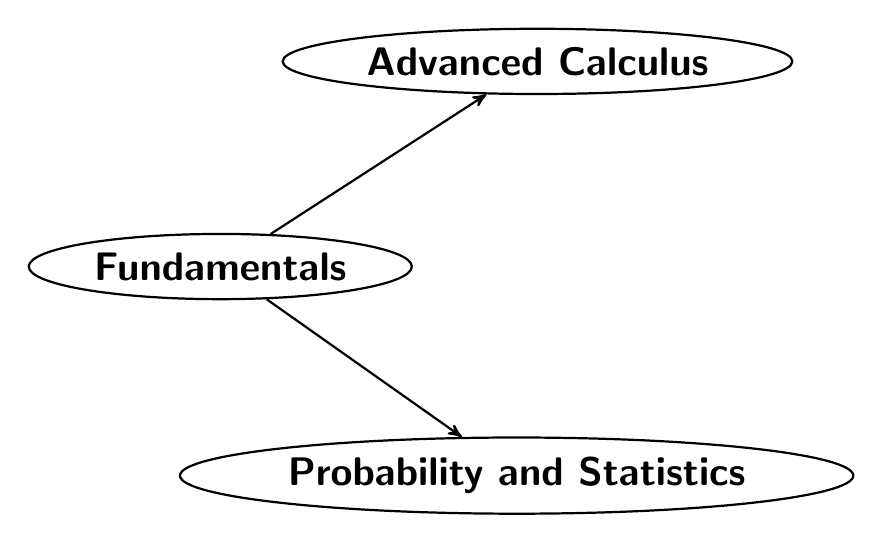
\begin{tikzpicture}[->,>=stealth',auto,thick,main node/.style={ellipse,draw,font=\sffamily\Large\bfseries}]
\node[main node] (a) {Fundamentals};
\node[main node] (b) [above right = 2cm and 0cm of a] {Advanced Calculus};
\node[main node] (c) [below right = 2cm and -1cm of a] {Probability and Statistics};

\draw[->] (a) -- (b);
\draw[->] (a) -- (c);
\end{tikzpicture}
\end{center}
\caption{Ideal High-Level Content Structure for the University of Adelaide Bridging Courses \label{fig:contentStructure}}
\end{figure}






\section{Further Research}

\begin{itemize}
	\item Complete a more comprehensive systematic review of the literature surrounding mathematics bridging and the secondary-tertiary transition.
	\item Review of Australian Universities, Bridging courses they offer, and placing the UofA courses into that context.
	\item Generation of Resources for a Probability and Statistics Topic booklet
	\item Alignment of final year highschool curriculum content internationally, and accross the other states of Australia in comparison to the \gls{ac}.
\end{itemize}


\begin{itemize}
	\item Developing a measure of ``granularity'' and estimating it's effect on learning could make for an interesting line of future research,
	\item This could indicate that the categorisation of concepts into these two content areas is not the most appropriate and maybe more appropriate content area groupings could be found for these topics, or perhaps more likely simply that these concepts are highly interconnected and so are often taught together in an integrated way. Exploring this in a broader sense, in terms of when concepts are taught separately and when they are integrated together could make for very interesting future research and very applicable to recent trends in educational research into \gls{stem}.
\end{itemize}

\begin{itemize}
	\item Foundational knowledge, assumed skills, looking at the year 10 curriculum and prior.
\end{itemize}

\begin{itemize}
	\item Broadly, a big difference in emphasis between the bridging courses and the \gls{ac}/ \gls{sace} is the emphasis the bridging courses place on sketching graphs, and explicitly exploring the connection between how transformations (translations and dilations primarily) of a graph relate to algebraic changes to functions. Although this is covered in \gls{sace} to some degree, it is largely implicit and left to reading between the lines, while it is quite explicit and fairly systematically embedded in the bridging courses. Whether this is an advantagous emphasis or not is beyond the scope of this work, but would make for interesting future research.
\end{itemize}

\begin{itemize}
	\item Review the old MT5, and map complex number concepts to the \gls{ac} and \gls{sace}.
\end{itemize}	


\begin{itemize}
	\item Longterm effects of Maths Anxiety Interventions.
\end{itemize}

% APPENDICES
\cleardoublepage
\begin{appendices}

\cleardoublepage
\chapter{Key-Concept Level Description of Topics}
\label{app:concepts}

Note, topics are identified using the code notation introduced in \reftab{notation}. The full \textbf{topic name is given in bold where applicable}, and then key concepts covered in that topic are listed.

% Giant Table of Key Concepts
\documentclass[varwidth=144mm, 12pt]{standalone}

% Multi-page Tables
\usepackage{longtable}

% Math
\usepackage{amsfonts}
\usepackage{amsmath}

% CMU sans serif font.
\usepackage[T1]{fontenc}
\renewcommand*\familydefault{\sfdefault}

% Hyperlinks
\usepackage{hyperref}

\begin{document}
\begin{longtable}{lp{.85\textwidth}}
Code & \textbf{Name} and Key Concepts \\ \hline
& \\ \endhead
%\multicolumn{2}{l}{\gls{ac} Senior Mathematical Methods} \\ 
MMu1t1 & \textbf{Functions and graphs}: Lines, Quadratics, Inverse Proportions, Polynomials, Relations, Translations and Dilations \\
MMu1t2 & \textbf{Trigonometric functions}: Unit Circle, Radians, SOH CAH TOA, Sine Rule, Exact Values, Amplitude/ Period/ Phase, Sum of Angles Identities \\
MMu1t3 & \textbf{Counting and probability}: Binomial Coefficients, Set Complement Intersection and Union, Probability, $P(A\cup{}B) = P(A) + P(B) - P(A\cap{}B)$, Conditional Probability, Independance \\
MMu2t1 & \textbf{Exponential functions}: Index Laws, Fractional Indices, Functions, Asymptotes, Graphs \\
MMu2t2 & \textbf{Arithmetic and geometric sequences and series}: Arithmetic and Geometric Sequences as Recurrence Relations, Limiting Behaviour, and Partial Sum Formulae, Growth and Decay \\
MMu2t3 & \textbf{Introduction to differential calculus} Average Rate of Change, First Principles, Leibniz Notation, Instantaneous Rate of Change, Slope of Tangent, Derivitive of Polynomials, Linearity of Differentiation, Optimisation, Anti-Derivitives, Interpret Position-Time Graphs \\
MMu3t1 & \textbf{Further differentiation and applications}: Define $e$ as $a$ s.t. $\lim_{h \to 0} \frac{a^h - 1}{h} = 1$, Derivitives of $e^x$ $\sin(x)$ and $\cos(x)$, Chain Product and Quotient Rules, Second Derivitives \\
MMu3t2 & \textbf{Integrals}: Integrate Polynomial Exponential and Trigonometric Functions, Linearity of Integration,  Determine Displacement given Velocity, Definite Integrals, Fundamental Theorem of Calculus, (signed) Area Under a Curve \\
MMu3t3 & \textbf{Discrete random variables}: Frequencies, General Properties, Expected Value, Variance, Standard Deviation, Bernoulli and Binomial Distribtions \\
MMu4t1 & \textbf{The logarithmic function}: Logs as Inverse of Exponentials, Log-Scales, Log Function Graphs, Natural Log, $\frac{d}{dx}\ln(x) = \frac{1}{x}$, $\int{\frac{1}{x}dx} = \ln(x) + c$ for $x > 0$ \\
MMu4t2 & \textbf{Continuous random variables and the normal distribution}: Probability Density Function, Cumulative Distribution Function, Probabilites Expected Value, Variance and Standard Deviation as Integrals, Linear Transformation of Random Variables, Normal Distribution using Technology \\
MMu4t3 & \textbf{Interval estimates for proportions} Simple Random Sampling, Bias, Sample Proportion, Normal Approximation to the Binomial Proportion, Wald Confidence Interval, Trade-Off Between Width and Level of Confidence \\
& \\
%\multicolumn{2}{l}{\gls{ac} Senior Specialist Mathematics} \\ 
SMu1t1 & \textbf{Combinatorics} Multiplication of Possibilities, Factorial Notation, Permutations with and without Repeated Objects, Union of Three Sets, Pigeon-Hole Principle, Combinations, Pascals Triangle \\
SMu1t2 & \textbf{Vectors in the plane}: Magnetude and Direction, Scalar Multiplication, Addition and Substraction as a Triangle, Vector Notation, $a\textbf{i} + b\textbf{j}$ Notation, Scalar Dot Product, Projection, Parallel and Perpendicular Vectors \\
SMu1t3 & \textbf{Geometry}: Notation for Implication ($\Rightarrow$) and Equivalence ($\Leftrightarrow$), Converse ($B \Rightarrow A$) Negation ($\neg A \Rightarrow \neg B$) and Contrapositive ($\neg B \Rightarrow \neg A$), Proof by Contradiction, $\forall$ and $\exists$ Notation, Counter-Examples, Circle Theorems, Quadrilateral Proofs in $\mathbb{R}^2$ \\
SMu2t1 & \textbf{Trigonometry}: Graph and Solve Trig Functions, Prove Various Trig Indentities, Reciprocal Trig Functions \\
SMu2t2 & \textbf{Matrices}: Notation, Addition and Scalar Multiplication of Matrices, Multiplicative Identity and Inverse, Determinant, Matrices as Transformations \\
SMu2t3 & \textbf{Real and complex numbers}: Rationality and Irrationality, Induction, $i = \sqrt{-1}$, Complex Numbers $a + bi$ and Arithmetic ($+$, $-$, $\times$, $\div$), Complex Conjugates, Complex Plane,  Complex Conjugate Roots of Polynomials \\
SMu3t1 & \textbf{Complex numbers}: Modulus and Argument, Arithmetic ($\times$, $\div$, and $z^n$) in Polar Form, Convert between Polar and Cartesian Form, De Moivre's Theorem, Roots of Complex Numbers, Factorising Polynomials \\
SMu3t2 & \textbf{Functions and sketching graphs}: Composition of Functions, One-to-One, Inverse Functions, Absolute Value Function, Rational Functions \\
SMu3t3 & \textbf{Vectors in three dimensions}: $a\textbf{i} + b\textbf{j} + c\textbf{k}$ Notation, Equation for Spheres, Parameterised Vector Equations, Equations of Lines, the Cross Product, Equation for a Plane, Systems of Linear Equation (Elimination Method) and Geometric Interpretation of Solutions, Kinematics via Differentiation of Vector Equations, Projectile and Circular Motion \\
SMu4t1 & \textbf{Integration and applications of integration} Substitution, $\int{\frac{1}{x}dx} = \ln{|x|} + c$ for $x \neq 0$, Inverse Trig Functions and their Derivitives, Integrate $\frac{\pm1}{\sqrt{a^2-x^2}}$ and $\frac{a}{a^2 + x^2}$, Partial Fractions, Integration by Parts, Volume of Solids of Revolution, Numerical Integration using Technology \\
SMu4t2 & \textbf{Rates of change and differential equations}: Implicit Differentiation, First-Order Seperable Differential Equations, The Logistic Equation, Kinematics (Rates of Change) \\
SMu4t3 & \textbf{Statistical inference}: Central Limit Theorem and the Resulting Confidence Interval for a Mean \\
& \\
%\multicolumn{2}{l}{\gls{sace} Stage 1 Mathematics} \\ 
S1M1 & \textbf{Functions and graphs}: Equations for a Line, Slope, y-intercept, Intersection of Lines, Reciprocal Function, Asymptotes, Functions vs Relations, Domain, Range, Function Notation \\
S1M2 & \textbf{Polynomials}: Quadratic Equations in Vertex and Factorised Forms, Quadratic Formula, Completing the Square, The Leading Coefficient and Degree of a Polynomials, Cubics, Quartics\\
S1M3 & \textbf{Trigonometry}: Pythagoras, SOH CAH TOA, Cosine Rule, Sine Rule, Unit Circle, Sine and Cosine Functions, Radians, Length of Arc, Area of Sector, Amplitude, Period, Phase, $\tan(x) = \frac{\sin(x)}{\cos(x)}$ \\
S1M4 & \textbf{Counting and statistics}: Factorial, Permutations, Multiplication Principle, Combinations, Discrete vs Continuous Random Variables, Mean, Median, Mode, Range, Interquartile Range, Standard Deviation, Normal Distribution, \\
S1M5 & \textbf{Growth and decay}: Index and Logarithm Laws, Exponential Functions and their Graphs \\
S1M6 & \textbf{Introduction to differential calculus}: Average Rate of Change, First Principles, Notation $f'(x) = \frac{df}{dx}$, $\frac{d}{dx}x^n = nx^{n-1}$, Linearity of Differentiation, Slope of Tangent, Increasing vs Decreasing, Local and Global Maxima and Minima, Stationary Points, Sign Diagram \\
S1M7 & \textbf{Arithmetic and geometric sequences and series}: Arithmetic and Geometric Series as Recurrance Relations and Explicit Expressions, Partial Sums, Limiting Behaviour  \\
S1M8 & \textbf{Geometry}: \href{https://prezi.com/view/vpmCHdeFbIV2xlYHhZiK}{Circle Properties}, Proofs (Direct, Contradiction, and Contrapositive) \\
S1M9 & \textbf{Vectors in the plane}: Component (column) vs $ai + bj$ Notation, Length and Direction, Linear Combinations of Vectors, Scalar Dot Product, Projection, Angle Between Two Vectors and Parallel/ Perpendicular, Geometric Proof \\
S1M10 & \textbf{Further Trigonometry}: Sketch Trigonometric Functions with Translations and Dilations, Solve for Angles, Trigonometric Identities, Reciprocal Trigonometric Functions\\
S1M11 & \textbf{Matrices}: Linear Combinations of Matrices, Matrix Multiplication, The Identity, Inverse Matrices, The $2 \times 2$ Inverse, The $2 \times 2$ Determinant, Linear Transformations (including rotations, reflections and composition) \\
S1M12 & \textbf{Real and complex numbers}: Rationals, Irrationals, Interval Notation, Induction, $i = \sqrt{-1}$, Real and Imaginary Components, Complex Conjugates and Arithmetic, Argand Diagram, Modulus, Complex Roots of Polynomals \\
& \\
%\multicolumn{2}{l}{\gls{sace} Stage 2 Mathematical Methods} \\ 
S2MM1 & \textbf{Further differentiation and applications}: S1M6, Chain Product and Quotient Rules, $e = 2.718\hdots$, $\frac{d}{dx}e^x = e^x$,  $\frac{d}{dx}\sin(x) = \cos(x)$, $\frac{d}{dx}\cos(x) = -\sin(x)$, Second Derivatives, Concavity and Points of Inflection \\
S2MM2 & \textbf{Discrete random variables}: Random Variables, Discrete vs Continuous, Probability Functions and Distributions, Properties of Probabilities, Frequency, Expected Value $E[X] = \sum{xp(x)} = \mu_X$, Standard Deviation $\sigma_X = \sqrt{\sum{(x-\mu_X)^2p(x)}}$, Uniform Bernoulli and Binomial Distributions \\
S2MM3 & \textbf{Integral calculus}: Anti-differentiation, If $F'(x) = f(x)$ then $\int{f(x)dx} = F(x) + c$, Reversing Chain Rule for $\int{f(ax + b)dx}$, Linearity of Integration, Finding the Constant of Integration, Area Under the Curve as Upper and Lower Sum Approximations, Definite Integral, Area Between Two Functions and Between a Negative Function and the x-axis, Fundamental Theorem of Calculus,  \\
S2MM4 & \textbf{Logarithmic functions}: Sketching $y = a\ln(b(x-c))$, $\frac{d}{dx}\ln(x) = \frac{1}{x}$, For $x > 0$ $\int{\frac{1}{x}dx} = \ln(x) + c$ \\
S2MM5 & \textbf{Continuous random variables and the normal distribution}: $P(X = x) = 0$, Probability Density Function, $\mu_X = \int_{-\infty}^{\infty}{xf(x)dx}$, $\sigma_X = \int_{-\infty}^{\infty}{(x - \mu_X)^2f(x)dx}$, $f(x) = \frac{1}{\sigma\sqrt{2\pi}}e^{-\frac{1}{2}\left( \frac{x-\mu}{\sigma}\right)^2}$, Standard Normal $Z = \frac{X - \mu}{\sigma}$, Simple Random Sampling, For $X \sim (\mu, \sigma)$ and $X_i \sim iid X$ Sampling Distributions of $S_n = \Sigma_{i = 1}^{n}{X_i}$ $(n\mu,\sigma\sqrt{n})$ and $\bar{X}_n = \frac{S_n}{n}$ $(\mu,\frac{\sigma}{\sqrt{n}})$, If $X$ is Normally Distributed, then so are $S_n$ and $\bar{X}_n$, Central Limit Theorem (CLT) \\
S2MM6 & \textbf{Sampling and confidence intervals}: Confidence Interval for a Mean using CLT $\left(\bar{x} - z^*\frac{s}{\sqrt{n}} \right) \leq \mu \leq \left( \bar{x} + z^*\frac{s}{\sqrt{n}}\right)$, Wald Interval for a Proportion  \\
& \\
%\multicolumn{2}{l}{\gls{sace} Stage 2 Specialist Mathematics} \\ 
S2SM1 & \textbf{Mathematical induction}: Initial Case and Induction Step \\
S2SM2 & \textbf{Complex numbers}: Cartesian vs Polar Form, Real and Imaginary Components, Modulus and Argument, Arithmetic in both Cartesian and Polar Forms, de Moivre's Theorem including Negative and Fractional Powers, Geometric Properties of the Argand Plane, Complex Arithmetic as Transformations, $n^{\text{th}}$ Roots of a Complex Number, Factorising Polynomials with Complex Roots \\
S2SM3 & \textbf{Functions and sketching graphs}: Function Composition, Informal Intro to Domain and Range, One-to-One, Inverse Functions, Absolute Value Function, Graphing Rational Functions \\
S2SM4 & \textbf{Vectors in three dimensions}: Notation, Equations of a Line in $\mathbb{R}^3$, Scalar Dot Product, Vector Cross Product, $|\mathbf{a} \times \mathbf{b}|$ is the Area of their Parallelogram, Equation for a Plane in $\mathbb{R}^3$, Systems of Linear Equations, Geometric Interpretation of No/Unique/Infinite Solutions to a System of Linear Equations in $\mathbb{R}^3$ \\
S2SM5 & \textbf{Integration techniques and applications}: Integration by Substitution, Using Trigonometric Identities for Integration, Derivatives of Inverse Trigonometric Functions (so $\int{\frac{\pm1}{\sqrt{a^2-x^2}}dx}$ and $\int{\frac{a}{a^2+x^2}dx}$, Integration by Parts, Area Between two Curves, Volume of Solids of Revolution \\
S2SM6 & \textbf{Rates of change and differential equations}: Implicit Differentiation, First-Order Seperable Differential Equations, The Logistic Differential Equation, Parameterised Curves, Example: if $\mathbf{v} = \frac{d}{dt}(x(t),y(t))$ is Velocity, $|\mathbf{v}|$ is Speed, and so the Arc Length along the Parameterised Curve is $\int_a^b{\sqrt{\mathbf{v} \bullet \mathbf{v}}dt}$, Trigonometric Parameterisations (unit circle, and non-circular parameterisations) \\
& \\
%\multicolumn{2}{l}{UofA MathStart} \\ 
MS1 & \textbf{Numbers \& Functions}: Natural Numbers, Integers, Rational Numbers, Real Numbers, Functions, Intervals \\
MS2 & \textbf{Linear Functions}: Equation for Linear Functions, Simultaneous Linear Equations, Sketching Linear Inequalities \\
MS3 & \textbf{Quadratic Functions}: Sketching a Parabola, General Form of a Quadratic, Translations and Dilations \\
MS4 & \textbf{Rational Functions}: Sketching Reciprocal Functions (Hyperbola), Lines of Symmetry, Limits and Asymptotes \\
MS5 & \textbf{Trigonometry I}: Pythagoras, Similar Triangles, SOH CAH TOA, Trigonometric and Inverse Trigonometric Functions using Technology, Exact Values\\
MS6 & \textbf{Trigonometry II}: Unit Circle, Sketching Trigonometric Functions, Finding all Solutions to Trigonometric Equations, The Sine Rule, The Cosine Rule, Introductory Trigonometric Identities, Radians \\
MS7 & \textbf{Exponential Functions}: Index Laws, Sketching Exponential Functions, $e = 2.718\hdots$, Growth and Decay\\
MS8 & \textbf{Logarithms}: Natural Logarithm, Logarithm Laws, Using Logarithm to Fit Growth/Decay Functions, Half-Life/ Doubling Time\\
& \\
%\multicolumn{2}{l}{UofA MathTrack} \\ 
MT1 & \textbf{Polynomials}: Polynomial Division and ``Remainder Theorem'', Factor Theorem Linking Zeros to Factors, Continuous vs Discontinuous Functions, Smoothness, Sketching Factorised Form of Polynomials, Factorising Polynomials, The Quadratic Formula \\
MT2 & \textbf{Matrices}: Order, Notation, Linear Combinations of Matrices, Matrix Multiplication (Associative but not Commutative, Distributes across Linear Combinations), The Identity Matrix, Powers of Square Matrices, Matrix Transpose, Systems of Linear Equations, Matrix Inverse, $2 \times 2$ determinant, The $2 \times 2$ Inverse, $n \times n$ Inverses, Elementary Row Operations, \\
MT3 & \textbf{Vectors and Applications}: Directed Line Segment Notation for Vectors, Magnetude/ Length and Direction, Linear Combinations of Vectors, Component and $a\mathbf{i} + b\mathbf{j}$ Notation, Vectors in $\mathbb{R}^2$ and $\mathbb{R}^3$, Scalar Dot Product, Equation for a Plane in $\mathbb{R}^3$ \\
MT4 & \textbf{Systems of Linear Equations}: Augmented Matrix for Systems of Linear Equations, Elementary Row Operations, Row-Echelon Form, Solutions to Systems of Linear Equations and Geometric Interpretations in $\mathbb{R}^2$ and $\mathbb{R}^3$, Matrix Inverses by Gauss-Jordan Elimination \\
MT6 & \textbf{Differentiation}: Rates of Change, Gradient, First Principles, Limit Notation, Derivative Notation, $\frac{d}{dx}x^n = nx^{n-1}$ (including $n = 0$ and $n = 1$), Linearity of Differentiation, Product Rule, Quotient Rule, Chain Rule, Implicit Differentiation, Normal to a Curve \\
MT7 & \textbf{Applications of Differentiation}: Sketching Polynomials and Rational Functions (Intercepts and Asymptotes), Continuity, Sign Diagrams, Increasing and Decreasing, Stationary Points, Points of Inflection, Concavity, Optimisation, \\
MT8 & \textbf{Exponential and Logarithm Functions}: Sketching Exponential Functions, $e = 2.718\hdots$, $\frac{d}{dx}e^x = e^x$, Natural Logarithm, $\frac{d}{dx}\ln(x) = \frac{1}{x}$, Growth and Decay, Surge Models, Logistic Models \\
MT9 & \textbf{Integration}: Area Under a Curve, Lower and Upper Sums, Definite Integrals, Definite Integrals of Negative Functions, Linearity of Integration, Properties of Definite Integrals, Fundamental Theorem of Calculus, Antiderivatives, Indefinite Integrals, Integrating by Reversing the Chain Rule, Integration by Substitution, Area Between two Curves, Summation Notation (Appendix) \\
\end{longtable}
\end{document}

\end{appendices}

% Bibliography/ References
\glsresetall
\cleardoublepage
\bibliographystyle{apacite}
\bibliography{citations} 

\end{document}


